%%%%%%%%%%%%%%%%%%%%%%%%%%%%%%%%%%%%%%%%%%%%%%%%%%%%%%%%%%%%%%%%%%%%%%
%% Torddis manuscript adapted to Education and Information Technologies
%% Springer Nature LaTeX template v3.1 (December 2024), APA reference style
%% Journal: Education and Information Technologies (EAIT)
%% ISSN: 1360-2357 (print), 1573-7608 (online)
%%%%%%%%%%%%%%%%%%%%%%%%%%%%%%%%%%%%%%%%%%%%%%%%%%%%%%%%%%%%%%%%%%%%%%
% APA Reference Style (EAIT uses APA 7)
\documentclass[pdflatex,sn-apa]{sn-jnl}

\usepackage[T1]{fontenc}
\usepackage[utf8]{inputenc}
\usepackage{graphicx}
\usepackage{multirow}
\usepackage{amsmath,amssymb,amsfonts}
\usepackage{amsthm}
\usepackage{mathrsfs}
\usepackage[title]{appendix}
\usepackage{xcolor}
\usepackage{textcomp}
\usepackage{manyfoot}
\usepackage{booktabs}
\usepackage{algorithm}
\usepackage{algorithmicx}
\usepackage{algpseudocode}
\usepackage{listings}
\usepackage{placeins}
\usepackage{array}
\usepackage{tabularx}
\usepackage{longtable}
\usepackage{pgfplots}
\usepackage{tikz}
\usepackage{subcaption}
\usepackage[export]{adjustbox}
\usepackage{url}

\pgfplotsset{compat=1.18}
\graphicspath{{figs/}}


\setlength{\extrarowheight}{2pt}%

%% Local helper macros used in the tables of the original manuscript
\newcommand{\datacell}[2]{\makebox[\linewidth][r]{#1\hspace{#2}}}%
\pgfmathsetmacro{\average}{81.46}%
\pgfmathsetmacro{\stdev}{11.65}%
\pgfmathsetmacro{\upperlimit}{\average+\stdev}%
\pgfmathsetmacro{\lowerlimit}{\average-\stdev}%

\raggedbottom%

\begin{document}

\title[Torddis for at-home learning]{Torddis: A Real-Time IoT and AI-Based System to Support At-Home Learning and Mitigate Parental Absenteeism}

%%=============================================================%%
%% Author metadata in Springer Nature format
%%=============================================================%%

%%=============================================================%%
%% Author metadata in Springer Nature format
%% ORCIDs are listed in the Author Contributions block within
%% Statements and Declarations, since the sn-jnl.cls class
%% intercepts \thanks and does not render them next to author
%% names on the title page.
%%=============================================================%%

%% Principal corresponding author (as in the original manuscript, cor1)
\author*[2]{\fnm{Miguel J.} \sur{Hornos}}\email{mhornos@ugr.es}

%% Secondary corresponding author (as in the original manuscript, cor2)
\author[1]{\fnm{Gleiston} \sur{Guerrero-Ulloa}}\email{gguerrero@uteq.edu.ec}

\author[1]{\fnm{Carlos} \sur{Almeida-Due\~nas}}\email{carlos.almeida2017@uteq.edu.ec}

\author[1]{\fnm{John} \sur{Plazarte-Su\'arez}}\email{john.plazarte2017@uteq.edu.ec}

\author[1]{\fnm{Orlando} \sur{Erazo-Moreta}}\email{oerazo@uteq.edu.ec}

\author[2]{\fnm{Carlos} \sur{Rodr\'iguez-Dom\'inguez}}\email{carlosrodriguez@ugr.es}

\affil[1]{\orgdiv{Faculty of Engineering Sciences},
    \orgname{State Technical University of Quevedo},
    \orgaddress{
        \street{Central Campus, Quito Avenue km. 1 1/2, on the way to Santo Domingo de los Ts\'achilas},
        \city{Quevedo},
        \postcode{120301},
        \state{Los R\'ios},
        \country{Ecuador}
    }
}

\affil*[2]{\orgdiv{Software Engineering Department, Research Centre for Information and Communication Technologies (CITIC-UGR), Aynadamar Campus},
    \orgname{University of Granada},
    \orgaddress{
        \city{Granada},
        \postcode{18071},
        \country{Spain}
    }
}

%%==================================%%
%% Unstructured abstract (150-250 words as per EAIT guidelines)
%%==================================%%

\abstract{
    Parental absenteeism during out-of-school study hours has intensified in recent years, undermining the academic performance and self-regulation of primary school children. This paper introduces Torddis, a real-time system that combines Internet of Things (IoT) hardware and Artificial Intelligence (AI) models to support at-home learning when tutors cannot provide continuous supervision. Torddis integrates an ESP32-CAM/NodeMCU device with a mobile application; it detects facial expressions indicative of inattention, unauthorised objects on the desk, and signs of drowsiness, and returns visual and auditory alerts that promote self-correction. The system was designed and validated following the Test-Driven Development Methodology for IoT Systems (TDDM4IoTS). A pilot deployment was carried out in twelve families in Quevedo, Ecuador, over one week; tutors evaluated the prototype through the System Usability Scale (SUS) and a purpose-built seven-item Likert questionnaire on perceived effectiveness. Torddis obtained a mean SUS score of 81.46\% (SD = 11.65), corresponding to a ``Good'' usability level. Statistical analyses (Shapiro--Wilk, ANOVA, Kruskal--Wallis, Pearson and Spearman correlations) revealed a strong positive association between the use of the device and tutor-perceived improvements in children's concentration and self-regulation. The findings support the pedagogical value of AI-enabled IoT tools for autonomous learning at home and outline avenues for larger and longer-term evaluations.
}

\keywords{Educational technology, Internet of Things, Artificial intelligence, Self-regulated learning, Home-based learning, Usability evaluation}

\maketitle

%%=========================================================================%%
%% Body of the manuscript
%% (Content preserved from the original manuscript; only the front matter,
%% references style, declarations block and appendix style were adapted to
%% EAIT/Springer Nature requirements.)
%%=========================================================================%%

\section{Introduction}
Over the last decade, accelerated lifestyles and increasing workloads have contributed to a rise in parental absenteeism during the hours designated for schoolwork at home, particularly among primary school students. This situation has underscored the need for technological solutions to compensate for the lack of supervision \citep{Seidu2022Truancy,Ketsman2025Mapping}.

The absence of parental support directly impacts the academic performance of young learners. Teachers have observed a decline in indicators related to performance and discipline, which may adversely affect students’ self-esteem and other psychosocial dimensions. Additionally, the literature emphasizes that emotional support in the home is a fundamental pillar for maintaining children’s focus on their studies \citep{Seidu2022Truancy}.

Emotional interference affects both educational outcomes and broader aspects of students’ lives \citep{Ake2023}. In this context, a family environment that fosters positive communication and genuine interaction can enhance students’ well-being and social skills \citep{Navarro2024}. However, to effectively address the challenges associated with attention and emotional regulation, it is crucial to incorporate technological tools that integrate Artificial Intelligence (AI) and the Internet of Things (IoT). These technologies enable the monitoring and measurement of children's distractions, providing essential data to support decision-making processes aimed at improving attention and learning outcomes \citep{Alvear-Puertas2017,Berrezueta-Guzman2021}.

The use of AI- and IoT-based technologies contributes to improved academic performance and to the development of self-regulation skills in students, which are essential for their cognitive and socio-emotional development \citep{Mohamed2018Implementing}. The feedback provided by such technologies helps students identify their distractions and take corrective actions, strengthening their ability to manage time and concentrate on academic tasks. Consequently, technological tools emerge as valuable resources to complement the positive influence of the family environment and to foster self-regulated learning, creating a comprehensive approach that encompasses both educational and personal development \citep{Thinyane2016AUG}.

Students' ability to concentrate is a crucial factor in their capacity to learn and apply knowledge delivered by educators. In a study conducted by \cite{Terraza2022}, a system was proposed to monitor students’ attention in an online learning environment using computer vision algorithms. The authors implemented a Recurrent Neural Network (RNN) to identify facial landmarks, detecting whether a student maintained a frontal position toward the device used to attend virtual classes. Their study reveals some limitations present in current proposals.

On the other hand, the work of \cite{Berrezueta-Guzman2021} introduced a robotic system designed to interact with children diagnosed with Attention Deficit Hyperactivity Disorder (ADHD), helping them correct unhealthy habits and inappropriate behaviors associated with this condition. Although effective within its specific scope, this system is exclusively oriented toward children with ADHD. Its generalized application may lead to disruptions for children without this condition, and it lacks notification, alert, or alarm functionalities to inform guardians about potential incidents.

To promote active guardian participation and enhance children’s emotional well-being, this paper introduces Torddis\footnote{From Latin \textit{\textbf{Tor}queo \textbf{d}iscerno \textbf{dis}cipulus}, meaning ``detection of deviation or change in the student’s attention.''}, a technological solution designed to monitor student behavior while they autonomously perform academic tasks at home, notifying guardians of any significant event and conveying to students the feeling that they are not alone. Alongside this, Torddis is capable of playing sounds, including personalized messages according to user preferences.

To achieve these objectives, Torddis employs advanced computer vision algorithms and deep learning techniques. The system includes a mobile application for guardians and an IoT device that analyzes children's behavior while they complete schoolwork independently. Developed following the TDDM4IoTS methodology \citep{Guerrero-Ulloa2020TDDM4IoTS}, Torddis features a holistic approach, enabling guardians to monitor and respond with low latency to signs of inattention. Key functionalities include the detection of facial expressions associated with core emotions, identification of drowsiness, and recognition of inappropriate use of distractive objects during academic activities. These features allow guardians to encourage their children to remain focused through the use of visual and auditory reinforcement cues \citep{Al-Gburi2023,Enadula2021,Terraza2022}.

Torddis is designed to strengthen metacognitive skills such as time management and sustained attention, which are essential components of modern autonomous learning. Its emphasis on proactive supervision addresses the need to support children during a critical stage of development, providing guardians with a valuable tool that complements traditional supervision at home and contributes to improving educational outcomes within this population.

The main contributions of this paper are the following: (i)~the design, implementation and empirical evaluation of Torddis, a real-time system that combines Artificial Intelligence (AI) and Internet of Things (IoT) technologies to monitor primary-school children while they perform academic tasks at home; (ii)~the integration, within a single unobtrusive device, of four purpose-built recognition modules---person (identity) recognition, facial-expression analysis, drowsiness detection and the identification of distractive objects during academic activities; (iii)~an explicit mapping of these functionalities to the three phases of Zimmerman's SRL model (see Table~\ref{tab:srl-mapping}), which allows the pedagogical role of Torddis to be articulated in theoretical rather than purely technical terms; (iv)~the application of the Test-Driven Development Methodology for IoT Systems (TDDM4IoTS) to the full engineering process, ensuring a systematic, traceable and reproducible development pipeline; and (v)~a two-tier interaction model in which the IoT device delivers visual and auditory reinforcement cues to the child with low latency, whilst the mobile application relays timely notifications to the guardian.

The remainder of this article is organised as follows. Section~\ref{section:second} develops the theoretical framework that grounds Torddis in the self-regulated learning tradition and articulates the pedagogical rationale of the system.  Section~\ref{section:third} presents a review of the most relevant related work published in the last ten years. Section~\ref{section:fourth} describes the design and development of the Torddis system, including the applied methodology, the hardware and software artefacts and the AI models used. Section~\ref{section:fifth} outlines the methodological design of the pilot study and its experimental validation. Section~\ref{section:sixth} reports the empirical results, including the usability evaluation, the recognition performance and the statistical analysis of the guardians' responses. Section~\ref{section:discussion} discusses the main findings and their pedagogical implications, and Section~\ref{section:eight} concludes the article and suggests avenues for future research.

\section{Theoretical Framework}
\label{section:second}
Torddis is grounded in three complementary bodies of literature that jointly define its pedagogical rationale: the theory of self-regulated learning (SRL), which characterises the cognitive and motivational processes a learner must orchestrate when studying autonomously \citep{Zimmerman2000Attaining, Panadero2017Review}; the evidence on parental absenteeism and guardian mediation, which explains why those processes are especially fragile when adult supervision at home is intermittent \citep{Seidu2022Truancy, Wang2025Cultivating}; and the growing use of Artificial Intelligence (AI) and the Internet of Things (IoT) as scaffolding technologies capable of delivering timely, unobtrusive support within the study session \citep{Wang2025Development, Ackermans2025Young}. This section develops each of these three pillars in turn and closes by mapping the concrete functionalities of Torddis onto the phases of the SRL model that the system is designed to support.

\subsection{Self-Regulated Learning and Zimmerman's Cyclical Model}
\label{sec:srl-model}
Torddis is grounded in the paradigm of self-regulated learning (SRL) \citep{Zimmerman2000Attaining, Panadero2017Review}. Under Zimmerman's social-cognitive account, SRL unfolds through three cyclical phases---\textit{forethought}, \textit{performance} and \textit{self-reflection}---that take place, respectively, before, during and after each learning episode. The forethought phase brings together task analysis processes (goal setting and strategic planning) and self-motivational beliefs (self-efficacy perceptions, outcome expectations, task interest). The performance phase encompasses self-control processes (attention focusing, self-instruction, task strategies) and self-observation processes (metacognitive monitoring and self-recording of progress). The self-reflection phase involves self-judgment (self-evaluation, causal attribution) and self-reaction (self-satisfaction and inferences that feed back into the next forethought phase), thereby closing the cycle \citep{Amaefule2025Childrens, Kleimola2025Promoting}. Recent qualitative work in EAIT has shown that both children in primary school \citep{Amaefule2025Childrens} and higher-education students \citep{Kleimola2025Promoting} recognise these phases and map them onto specific expectations that they hold of any educational technology that claims to support their studying.

Zimmerman's framing is pedagogically actionable rather than merely descriptive: self-regulation is a set of competencies that can be explicitly taught and that consolidate through cyclical practice \citep{Zimmerman2002Becoming}. This distinction matters for the population Torddis targets, since meta-analytic evidence shows that structured SRL interventions already yield positive effects on strategy use and achievement at the primary- and secondary-school levels, with the strongest gains when the training is theory-grounded and embeds metacognitive prompts within authentic tasks \citep{Dignath2008Components}; comparable meta-analytic improvements in performance, strategy use and motivation have been reported for higher-education students \citep{Theobald2021Self}. Locating Torddis within this tradition implies that its cues should not substitute for the learner's regulatory work but scaffold the phase-specific subprocesses that such training targets, ideally fading as the child internalises them.

\subsection{Parental Absenteeism and Guardian Mediation of At-Home Learning}
\label{sec:guardian-mediation}
The home is the primary setting in which primary-school children consolidate these regulatory competencies, and the degree of adult involvement is a well-established correlate of their academic outcomes. Review and meta-analytic evidence links specific dimensions of parental involvement---shared reading, high but realistic expectations, and academic socialisation rather than mere homework surveillance---to measurable gains in achievement \citep{Boonk2018Review, Hill2009Parental}, whereas the erosion of that involvement through parental absence is associated with declining attendance and performance \citep{Seidu2022Truancy}. When guardians cannot be continuously present during study hours, the regulatory scaffolding that involvement normally supplies is precisely what is withdrawn.

When adult supervision is unavailable at home, self-regulation is precisely the skill children of primary-school age are still consolidating. Throughout this paper, we use the term \textit{guardian} to denote any adult who assumes responsibility for the child's academic activities at home, including biological or adoptive parents, legal guardians, grandparents, older siblings acting in a caregiving role, or any other primary caregiver. Complementary evidence from primary-school samples indicates that both restrictive and active parental mediation and, more decisively, environmental, capacity and metacognitive parental support shape children's online SRL by way of technological self-efficacy and perceived usefulness \citep{Wang2025Cultivating,An2024Relationship}. Children themselves, however, articulate consistent preferences: they want educational technology that helps them \textit{organise} their study (planning, scheduling, prompting), \textit{focus} on the learning task at hand (distraction management, atmosphere), and remain engaged through features that are attractive and rewarding \citep{Amaefule2025Childrens}. Moreover, the impact of such extramural technological factors on academic performance and well-being differs according to the child's self-regulatory profile, so an equivalent gap in home support does not translate into equivalent effects across learners \citep{Chen2024Extramural}.

\subsection{AI- and IoT-Mediated Scaffolding of Self-Regulation}
\label{sec:ai-iot-scaffolding}
AI-mediated feedback loops can scaffold this process by delivering timely, personalised cues that steer attention back to task \citep{Wang2025Development, Li2024Systematic}, and IoT devices are especially well suited to unstructured domestic settings because of their unobtrusive form factor \citep{Ackermans2025Young}. Torddis integrates these two threads: it uses AI models to detect emotional, cognitive and contextual signs of distraction, and it delivers personalised alerts within the study session, using IoT hardware chosen for its unobtrusive form factor. In doing so, it acts as a mediator between student autonomy and external guidance, supporting the development of digital competence and academic self-management \citep{Loh2025Plugging, Mohamed2018Implementing, Echeverria2011AFramework}.

These two technological threads are supported by maturing bodies of review evidence. Systematic reviews of Artificial Intelligence in education converge on adaptive personalisation, automated assessment and intelligent tutoring as the dominant application clusters, while cautioning that pedagogical grounding and critical reflection on risks still lag behind technical capability \citep{ZawackiRichter2019Systematic, Wang2025Development}. Reviews of IoT in education, in turn, report a rapid uptake of embedded, sensor-based devices alongside recurrent concerns about privacy, security and classroom integration \citep{Kassab2020Systematic}, and evidence specific to early-childhood and primary settings stresses that the value of such devices hinges on an unobtrusive, developmentally appropriate form factor \citep{Ling2022Use}. Torddis is deliberately positioned at this intersection: it operationalises the adaptive-feedback function emphasised in the AI literature through an IoT artefact shaped to the domestic, low-supervision context that the IoT-in-education reviews identify as comparatively underserved.

\subsection{Mapping Torddis Functionalities to the SRL Phases}
\label{sec:srl-mapping-section}
Table~\ref{tab:srl-mapping} summarises how the concrete functionalities of Torddis are theoretically anchored in Zimmerman's three-phase SRL model. In the \textit{forethought} phase, the physical presence and initial configuration of the Torddis IoT device act as an environmental cue that marks the transition into study, and the child's negotiated agreement with the guardian about session duration operates as a lightweight goal-setting scaffold in line with the planning support that primary-school children explicitly request \citep{Amaefule2025Childrens}. In the \textit{performance} phase, three of Torddis' AI modules directly address the self-control and self-observation processes highlighted by Zimmerman: facial-expression analysis externalises metacognitive monitoring of emotional engagement, drowsiness detection assists in the regulation of on-task attention, and distractive-object detection materialises the ``distraction management'' need that children voice as central \citep{Amaefule2025Childrens}. The auditory and visual reinforcement cues delivered by the device close the performance-phase loop by nudging the learner back to task without requiring the guardian's continuous presence. In the \textit{self-reflection} phase, the event logs generated by Torddis and the guardian's mobile-application notifications constitute an external record of performance that supports self-evaluation and joint reflection with the guardian---an operation analogous to what \citet{Kleimola2025Promoting} report for learning-analytics dashboards used in student-guardian guidance meetings, where visualised traces of learner behaviour become the shared object of attribution and next-cycle planning.

\begin{table}[!htbp]
	\centering
	\caption{Theoretical mapping of Torddis functionalities to the three phases of Zimmerman's self-regulated learning model.}
	\label{tab:srl-mapping}
	\setlength{\tabcolsep}{5pt}
	\begin{tabular}{
			>{\raggedright\arraybackslash}p{2.0cm}
			>{\raggedright\arraybackslash}p{4.0cm}
			>{\raggedright\arraybackslash}p{6.0cm}
		}
		\toprule
		\textbf{SRL phase} & \textbf{Zimmerman subprocesses} & \textbf{Torddis functionality that scaffolds them} \\
		\midrule
		Forethought & Task analysis; goal setting; strategic planning; self-motivational beliefs & Physical presence of the IoT device as environmental cue for study onset; guardian--child agreement on session duration registered in the mobile application \\
		Performance & Self-control (attention focusing, task strategies); self-observation (metacognitive monitoring, self-recording) & Facial-expression analysis (emotional engagement); drowsiness detection (on-task attention); distractive-object detection (behavioural focus); immediate visual and auditory reinforcement cues \\
		Self-reflection & Self-judgment (self-evaluation, causal attribution); self-reaction; adaptive inferences & Session-level event logs (alerts, active-supervision time, latencies); guardian notifications through the mobile application supporting joint post-session reflection \\
		\bottomrule
	\end{tabular}
\end{table}

This explicit mapping is important for two reasons. First, it repositions Torddis from a monitoring artefact to a scaffold that operates on documented SRL subprocesses, allowing hypotheses about its pedagogical effects to be formulated in terms of specific phases rather than diffuse ``improvements in concentration''. Second, it aligns Torddis with the design orientation that dominates recent EAIT contributions on SRL support technologies, in which functionalities are justified against theoretical phases and empirically evaluated with respect to how users perceive them addressing each phase \citep{Amaefule2025Childrens, Kleimola2025Promoting}. It must be stressed, however, that this mapping is a \emph{design rationale} that remains to be empirically validated: the pilot reported here measures guardian-perceived global effectiveness and usability, not the phase-specific forethought, performance and self-reflection subprocesses themselves, so the phase-level hypotheses it articulates are advanced for future testing rather than established in this study.

\section{Related Works}
\label{section:third}
The literature on the use of technologies for detecting and correcting student distractions is limited, particularly regarding the integration of IoT technologies for pedagogical purposes. Previous studies have addressed technological applications in child monitoring, yet few have explored how these technologies can be used to provide immediate feedback that promotes learning self-regulation and enhances educational outcomes in non-formal contexts. The state-of-the-art review process was conducted in accordance with the guidelines established by \cite{Kitchenham2007Guidelines}, whose methodology is presented in the diagram in Figure~\ref{fig:LRS}.

\begin{figure}[!htbp]
	\centering
	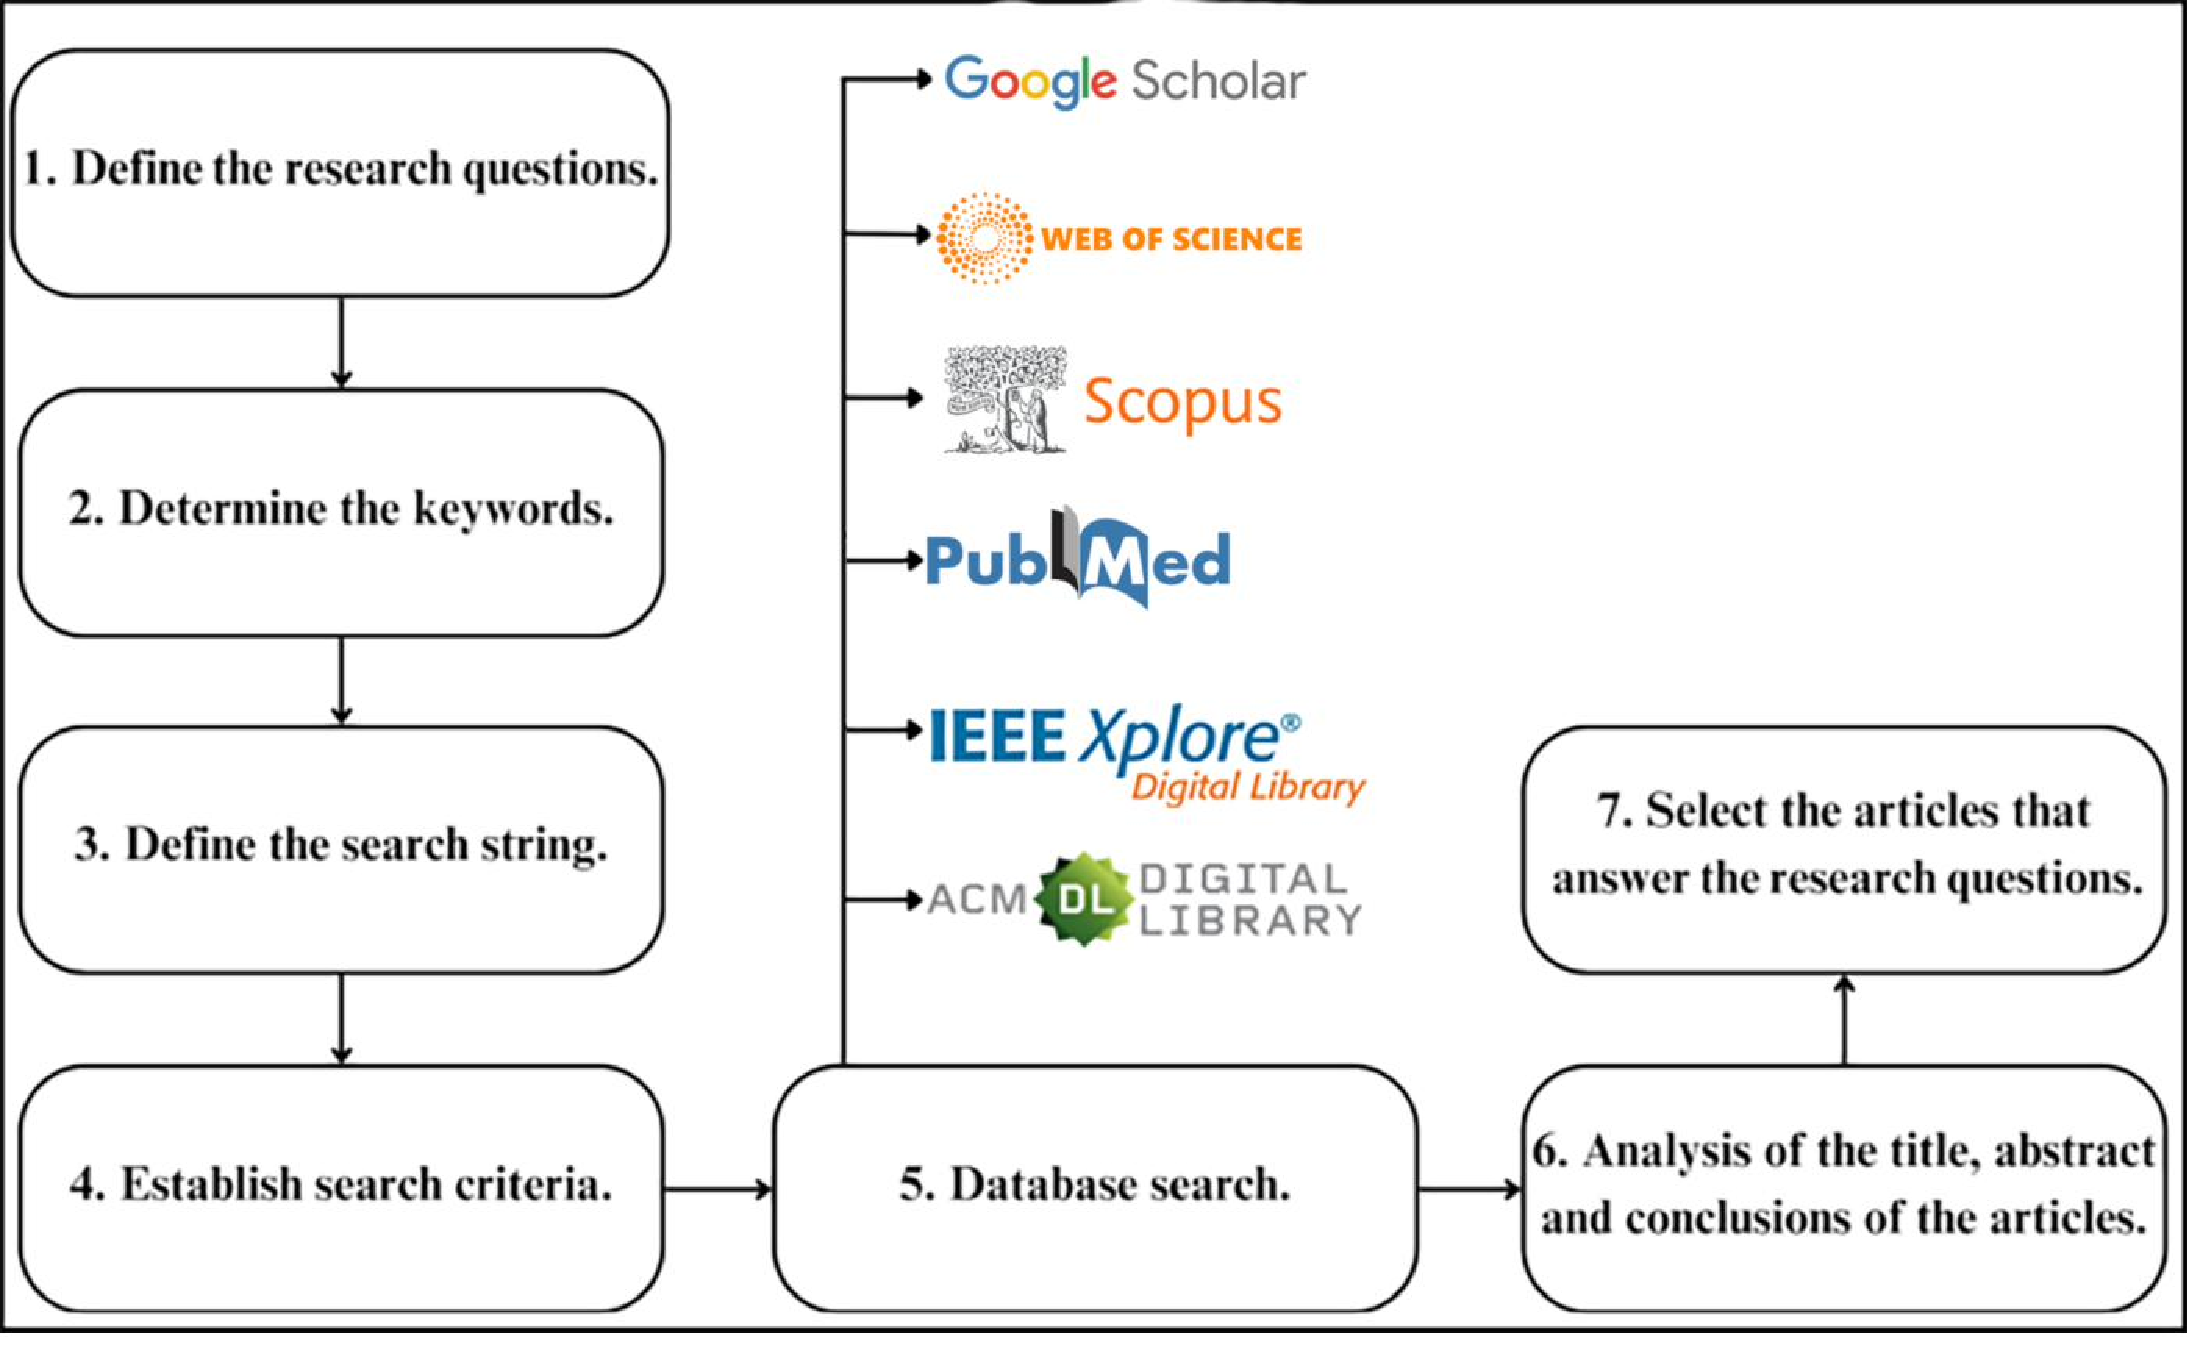
\includegraphics[width=\textwidth]{Figure_1}
	\caption{PRISMA-style flow diagram of the study identification, screening, eligibility and inclusion process across the five bibliographic databases, following \citet{Kitchenham2007Guidelines}. Counts correspond to Table~\ref{tab:Results}.}
	\label{fig:LRS}
\end{figure}

\subsection{Research Questions}
This article addresses the critical issue of detecting student distractions during autonomous schoolwork. With the increasing availability of digital tools for education and the growing need for effective learning strategies, understanding how distractions impact student performance has become essential. The following research questions guide this comprehensive review of related works and inform the development of technological solutions aimed at improving children’s concentration and educational outcomes:

\begin{itemize}
	\item \textit{RQ1:} Which AI and IoT technologies are most suitable for designing a system capable of monitoring children’s distractions during their school activities at home?
	
	\item \textit{RQ2:} What internal and external parameters can be used to detect distractions in children, and how should these be integrated into an IoT system to ensure effectiveness and personalization?
	
	\item \textit{RQ3:} How can a real-time IoT system foster key skills such as self-regulation, autonomous learning, and concentration in students working on school tasks at home?
	
	\item \textit{RQ4:} What are parents’ or guardians’ perceptions regarding the usefulness, usability, and effectiveness of an IoT system designed to support home learning, and how does this perception influence its acceptance?
\end{itemize}

\subsection{Search Strategy}
Once the research questions were defined, relevant keywords were selected to retrieve the most recent publications from major scientific databases in this research field. These keywords were used to construct the search string, which was then adapted to the specific requirements of each selected database. The final search string was: (distraction OR distractions) AND (child OR children OR student) AND (homework OR ``school assignments'' OR ``school tasks'') AND (''object recognition´´ OR ``facial recognition'' OR ``gesture recognition'').

The literature searches were conducted in five high-prestige scientific databases: ACM (Association for Computing Machinery) Digital Library, IEEE (Institute of Electrical and Electronics Engineers) Xplore, PubMed, Scopus, and Web of Science. These platforms facilitated the identification of pertinent literature using predefined criteria.

The database searches returned 4{,}881 records (Table~\ref{tab:Results}). After removing 953 duplicates, 3{,}927 records were screened by title and abstract, and 591 were assessed for eligibility. Applying the eligibility criteria---exclusion of non-study records (patents, grants and theses), records published before 2015, records without a DOI, records not presenting a system aligned with the objectives of this study, and records outside the target scope (detection only, without real-time intervention, a dedicated IoT device, or a home/self-regulation orientation)---yielded 70 included studies. The complete identification, screening, eligibility and inclusion process is depicted in the PRISMA-style flow diagram in Figure~\ref{fig:LRS}.

\begin{table}[!htbp]
	\caption{Records identified per database and studies finally included after screening and eligibility assessment (see Figure~\ref{fig:LRS}).\label{tab:Results}}
	\centering
	\begin{tabular*}{\linewidth}{@{\extracolsep{\fill}}
			>{\raggedright\arraybackslash}p{5cm}
			>{\raggedleft\arraybackslash}p{3cm}<{\hspace*{8pt}}
			>{\raggedleft\arraybackslash}p{3cm}
			@{}}
		\toprule
		\multicolumn{1}{c}{\textbf{Database}} &
		\multicolumn{1}{c}{\textbf{\shortstack{Records\\identified}}} &
		\multicolumn{1}{c}{\textbf{\shortstack{Studies\\included}}} \\
		\midrule
		ACM Digital Library & 1\,000 & 5 \\
		IEEE Xplore & 763 & 31 \\
		PubMed & 7 & 0 \\
		Scopus & 2\,148 & 33 \\
		Web of Science & 963 & 1 \\
		\midrule
		\textbf{Total} & \textbf{4\,881} & \textbf{70} \\
		\bottomrule
	\end{tabular*}
\end{table}

To ensure the transparency and reproducibility of this review, the search string adapted to each database, the complete set of retrieved records together with their screening and eligibility decisions (inclusion/exclusion and reason), and the data underlying the PRISMA flow diagram (Figure~\ref{fig:LRS}) are provided as Online Resource~2 (Supplementary Information) and deposited, under the same DOI as the rest of the study artefacts, in the Torddis reproducibility repository (see the \textit{Data Availability} statement), in line with the protocol of \citet{Kitchenham2007Guidelines}.

\subsection{Literature Analysis}
In the scientific literature on technologies applied to the fields of education and child care, several approaches focus on the use of Artificial Intelligence (AI), the Internet of Things (IoT), and computer vision techniques to enhance learning and behavioral monitoring. Additionally, other studies have integrated these technologies to facilitate learning self-regulation, improve concentration, and foster academic engagement across different student populations.

\subsubsection{Behavior Monitoring}
Studies such as those by \cite{Akter2021}, \cite{Albrecht2014}, \cite{Berrezueta-Guzman2021}, \cite{Pelc2006}, \cite{VilliersRader2021}, \cite{Warren2015Brief}, and \cite{Washington2016AWereable} explore applications ranging from early diagnosis of Autism Spectrum Disorder (ASD) to improving emotion recognition in children with Attention Deficit Hyperactivity Disorder (ADHD). These studies employ advanced technologies such as AI and connected devices to analyze and respond to specific child behaviors in both controlled and everyday environments.

For example, \cite{Akter2021} apply transfer learning\footnote{\textit{Transfer learning \cite{Akter2021}} refers to the extent to which learners can effectively and consistently apply the knowledge, skills, and attitudes acquired during a training activity to different contexts beyond the original learning environment. In essence, it assesses whether an educational experience promotes learning that can be generalized and sustained in real-life situations.} for ASD diagnosis through facial recognition. Similarly, \cite{Pelc2006} focus on recognizing emotions in children with ADHD using validated photographs, while \cite{Albrecht2014} investigate visual search strategies in children with ASD. \cite{Berrezueta-Guzman2021} evaluate the use of a robotic assistant to support academic tasks for children with ADHD, and \cite{VilliersRader2021} examine how gestures can direct attention toward word-object relationships in children with ASD.

Other studies, such as \cite{Boumiza2017}, \cite{DaCosta2023}, \cite{Enadula2021}, \cite{Farsani2020}, \cite{Hachad2020}, \cite{James2019}, \cite{Kulkarni2023}, \cite{Kumar2024Zoom}, \cite{Muller2018ArchnSmile}, \cite{Narkhede2023}, and \cite{Ozdamli2022}, also address issues related to safety, engagement, and interaction through monitoring technologies. For instance, \cite{Hachad2020} and \cite{James2019} employ facial recognition to monitor student safety on school buses and attendance in classrooms, respectively. Likewise, \cite{Ozdamli2022} use computer vision technologies to recognize emotions and detect cheating during online exams.

In addition, \cite{Campbell2015Using} and \cite{Ucar2022Recognizing} present systems designed to monitor distractions with low latency. For example, \cite{Campbell2015Using} use multispectral imaging to detect distractions caused by mobile devices, while \cite{Ucar2022Recognizing} employ facial recognition and head pose estimation to assess student engagement in virtual classes. Other works such as \cite{Argel2023Intellitell}, \cite{Erazo2016Easing}, and \cite{Nguyen2019} also focus on behavioral evaluation using advanced technologies like YOLOv3 for in-session monitoring and dynamic adjustment of teaching strategies.

Finally, studies such as \cite{Boumiza2017} and \cite{DaCosta2023} explore monitoring in contexts such as automated tutoring systems and school transportation within smart cities, highlighting the use of facial recognition to personalize educational experiences and enhance safety.

A systematic update of the literature (see Figure~\ref{fig:LRS} and Table~\ref{tab:Results}) retrieved a substantial body of recent work that monitors learners' states through computer vision, physiological sensing and machine learning. Within this group, a large share detects engagement or affective state from facial expressions \citep{Alalwani2016Combined, Wang2018Attention, Ashwin2020Impact, Yu2021Measuring, R2022Drowsiness, Daksith2023Multi, Prince2024Investigating, Qi2024Evaluation, K2025Capture, R2026Emotion, Singh2026Utilizing}, while others estimate attention, concentration or distraction from gaze, head-pose or behavioural cues \citep{Robal2018WebcamBased, Rk2020RealTime, Lee2022Wedar, Xu2024Identifying, Barrial2025Tool, Ramana2025Challenges, B2025Yolov8Based, Hanif2025RealTime, Bhimavarapu2025Leveraging}. Drowsiness or fatigue detection is addressed by \citep{R2022Drowsiness, Wang2022Online, Ramana2025Challenges, Nirosha2025Drowsiness, Hanif2025RealTime, Singh2026Utilizing}, and the identification of distractive objects such as mobile phones by \citep{Xu2024Identifying, B2025Yolov8Based, Singh2026Utilizing}. These works confirm the technical feasibility of automatic monitoring but, in general, stop at measurement and are oriented to the classroom or to online proctoring rather than to unsupervised study at home.

\subsubsection{Technology for Autonomous Learning}
Other studies focus on promoting self-regulation, concentration, and academic engagement by integrating technologies that support autonomous learning in diverse contexts. For instance, \cite{Bembich2016Future} investigate the use of digital technologies for future educators, providing self-regulation strategies to manage distractions. Similarly, \cite{Peters2003Self} examine how hypertext environments can improve volitional control and distraction management in digital autonomous learning.

\cite{Roberts2020Task} analyze how secondary students use digital records to self-regulate and reflect on their academic progress. On the other hand, \cite{Adcroft2018Developing} combine digital technologies with time management and mindfulness practices to help students improve their focus and self-regulation in daily tasks.

Studies such as \cite{Salter2014Exploring} and \cite{Palmer2022impact} integrate technologies and platforms to monitor and assess self-regulation skills. While \cite{Salter2014Exploring} adopt a whole-school approach, \cite{Palmer2022impact} focus on synchronous hybrid teaching in a pharmacotherapy course.

\cite{Muljana2022Instructional} and \cite{Wang2022Empowering} explore specific strategies to promote self-regulation. \cite{Muljana2022Instructional} analyze how instructional professionals use social media to develop self-directed learning, while \cite{Wang2022Empowering} investigate the reduction of digital distractions among university students through self-regulation skills.

A parallel line of enquiry, followed by \cite{Hartley2022Smartphone} and \cite{Labar2019Interplay}, examines the impact of mobile device use on attention and multitasking. While \cite{Labar2019Interplay} take a psychological approach to analyze time perception, \cite{Hartley2022Smartphone} focus on how smartphone use directly affects self-regulation abilities.

These studies reflect a diverse range of approaches to self-regulation and the improvement of autonomous learning, employing technological strategies to reduce distractions, enhance volitional control, and foster academic engagement.

A second group of recent studies identified in the systematic review is oriented to autonomous, self-regulated or at-home learning, using sensing and AI to support the learner's own regulation rather than external supervision \citep{Huang2021Student, Chen2023Mirrorus, Lathaharan2023Transforming}. These contributions align with the pedagogical goal pursued by Torddis---sustaining concentration during independent study---but most of them either lack a real-time corrective loop or are not embodied in an unobtrusive device suitable for the domestic setting.

\subsubsection{Real-Time Intervention and IoT-Based Systems}
Closest to the Torddis proposal is a third group of works, retrieved by the systematic review, that close the perception--action loop, either by issuing real-time interventions (alerts, cues, notifications or adaptive feedback) or by embedding the recognition pipeline in a dedicated IoT, edge or wearable device. Systems that react in real time to redirect the learner's attention or to notify a guardian or teacher are reported by \citep{Kim2018RealTime, Yeh2020Environmentally, Tennakoon2021EPod, Roy2021Students, Parthiban2021Emotion, Le2022Desk, Lopezcarreno2022University, Lopezcarreno2022ArtificialIntelligenceBased, Liu2022Enabled, Lee2022Measurements, Poonja2023Engagement, Berrezuetaguzman2023Artificial, Lee2023BehaviorBased, Costa2024Iot, Sudharsan2024Behavior, Rs2025Engage, Abbes2025Internet, Dhepe2025RealTime, Muthulingam2025Inclusive, Mohamed2025EmotionAware, Shiny2025Neurolearn, Sandhya2025LearningBased, Wang2025IotEnabled, Baheti2025Languages, Cao2026Yolov8Based, Guo2026RealTime, D2026Intellimentor, Huong2026Personalized, Ayyadurai2026Efficient}, whereas deployments on dedicated IoT/edge hardware (e.g., Raspberry Pi, Jetson, ESP32 or embedded cameras) are described by \citep{Kim2018RealTime, Yeh2020Environmentally, Abdo2021Attention, Parthiban2021Emotion, Henry2021Randomised, Le2022Desk, Ejaz2022RealTime, Liu2022Enabled, Mandia2023YoloV5, Poonja2023Engagement, Berrezuetaguzman2023Artificial, Abdulkader2023Optimizing, Elmugamer2024Evaluating, Costa2024Iot, Li2024Research, Sudharsan2024Behavior, Ami2025Student, Abushahla2025RealTime, Souhir2025Edge, Sandhya2025LearningBased, Huang2025Facial, Wang2025IotEnabled, Xu2025IotBased, Baheti2025Languages, Cao2026Yolov8Based, Guo2026RealTime, Thaseen2026Iot, Waheed2026Iot, Chen2026Iot, He2026Multimodal}. A subset explicitly targets the home or self-regulated setting \citep{Berrezuetaguzman2023Artificial, Ayyadurai2026Efficient}. Even within this most advanced group, however, no single system simultaneously integrates facial-expression, drowsiness and distractive-object recognition with an in-situ visual/auditory intervention and a guardian-facing mobile application in the domestic context, which is precisely the gap that Torddis addresses.

\subsubsection{Comparison of Torddis with Previous Works}
The literature analysis reveals significant progress in the use of advanced technologies to address educational and child care challenges. However, Torddis stands out as a comprehensive solution that integrates IoT, computer vision, and AI to deliver adaptive and proactive supervision in various environments. The following comparison outlines how Torddis overcomes limitations identified in the reviewed references. Table~\ref{tab:comparison} summarises this comparison across seven functional dimensions for a representative subset of the reviewed systems, showing that Torddis is the only one that combines in-session real-time intervention in the domestic setting with distractive-object, drowsiness and facial-expression recognition, guardian notification and an explicit self-regulated-learning grounding.

\begin{table}[!htbp]
	\centering
	\caption{Feature comparison of Torddis with representative reviewed systems. The classification follows each system's description in Section~\ref{section:third} and its cited source.}
	\label{tab:comparison}
	\setlength{\tabcolsep}{4pt}\footnotesize
	\begin{tabular*}{\linewidth}{@{\extracolsep{\fill}}>{\raggedright\arraybackslash}p{4.6cm}ccccccc@{}}
		\toprule
		\textbf{System} & \textbf{RTI} & \textbf{Home} & \textbf{Obj} & \textbf{Drw} & \textbf{Emo} & \textbf{Ntf} & \textbf{SRL} \\
		\midrule
		\citet{Berrezueta-Guzman2021}      & \checkmark & -- & -- & -- & -- & -- & -- \\
		\citet{Terraza2022}                & -- & -- & -- & -- & \checkmark & -- & -- \\
		\citet{Ucar2022Recognizing}        & -- & -- & -- & -- & \checkmark & -- & -- \\
		\citet{Campbell2015Using}          & -- & -- & \checkmark & -- & -- & -- & -- \\
		\citet{Argel2023Intellitell}       & -- & -- & -- & -- & \checkmark & -- & -- \\
		\citet{Ozdamli2022}                & -- & -- & -- & -- & \checkmark & -- & -- \\
		\textbf{Torddis (this work)}       & \checkmark & \checkmark & \checkmark & \checkmark & \checkmark & \checkmark & \checkmark \\
		\bottomrule
	\end{tabular*}
	\vspace{0.3em}
	\parbox{\linewidth}{\footnotesize
		RTI: in-session real-time intervention; Home: domestic (home) deployment; Obj: distractive-object detection; Drw: drowsiness detection; Emo: facial-expression/emotion recognition; Ntf: guardian notification/alert; SRL: explicit self-regulated-learning grounding. \checkmark~= present; --~= absent or not reported.
	}
\end{table}

While Table~\ref{tab:comparison} contrasts Torddis with a representative subset, the complete set of 70~studies retrieved by the systematic review is mapped in Table~\ref{tab:comparison-full} across the seven capabilities that Torddis integrates: facial-expression/emotion recognition (FE), drowsiness/fatigue detection (DR), distractive-object detection (OB), attention/engagement estimation (AT), real-time in-situ intervention (IN), deployment on a dedicated IoT/edge device (IoT) and an explicit home/self-regulation orientation (HM). The classification was verified against the full text of 64 of the 70 studies (the remaining six, marked $^{\dagger}$ in Table~\ref{tab:comparison-full}, were classified from title and abstract because their full text was unavailable). The mapping confirms that, although each individual capability is well represented in the recent literature, none of the 70~reviewed systems covers the seven dimensions simultaneously, whereas Torddis does.

\begin{longtable}{@{}>{\raggedright\arraybackslash}p{5.2cm}ccccccc@{}}
	\caption{Systematic comparison of the 70 studies selected through the review with Torddis across seven capabilities, verified against the full text of each study. FE: facial-expression/emotion; DR: drowsiness/fatigue; OB: distractive-object; AT: attention/engagement; IN: real-time in-situ intervention; IoT: dedicated IoT/edge device; HM: home/self-regulation orientation. Entries marked $^{\dagger}$ were classified from title and abstract because their full text was not available.\label{tab:comparison-full}}\\
	\toprule
	\textbf{Study} & \textbf{FE} & \textbf{DR} & \textbf{OB} & \textbf{AT} & \textbf{IN} & \textbf{IoT} & \textbf{HM} \\ \midrule
	\endfirsthead
	\toprule \textbf{Study} & \textbf{FE} & \textbf{DR} & \textbf{OB} & \textbf{AT} & \textbf{IN} & \textbf{IoT} & \textbf{HM} \\ \midrule \endhead
	\citet{Alalwani2016Combined} & \checkmark & -- & -- & \checkmark & -- & \checkmark & -- \\
	\citet{Robal2018WebcamBased} & -- & -- & -- & \checkmark & -- & -- & \checkmark \\
	\citet{Wang2018Attention} & \checkmark & \checkmark & -- & \checkmark & -- & -- & -- \\
	\citet{Rk2020RealTime} & \checkmark & \checkmark & -- & \checkmark & \checkmark & -- & -- \\
	\citet{Ashwin2020Impact} & \checkmark & \checkmark & -- & \checkmark & \checkmark & -- & -- \\
	\citet{Yu2021Measuring} & \checkmark & -- & -- & \checkmark & \checkmark & -- & -- \\
	\citet{Lee2022Wedar} & -- & -- & -- & \checkmark & -- & -- & \checkmark \\
	\citet{R2022Drowsiness} & \checkmark & \checkmark & -- & -- & -- & \checkmark & -- \\
	\citet{Wang2022Online} & -- & \checkmark & -- & -- & \checkmark & -- & -- \\
	\citet{Daksith2023Multi} & \checkmark & -- & -- & \checkmark & \checkmark & -- & -- \\
	\citet{Prince2024Investigating} & \checkmark & -- & -- & -- & \checkmark & -- & -- \\
	\citet{Qi2024Evaluation} & \checkmark & \checkmark & \checkmark & \checkmark & \checkmark & -- & -- \\
	\citet{Xu2024Identifying} & -- & -- & \checkmark & \checkmark & -- & -- & -- \\
	\citet{Barrial2025Tool} & -- & -- & -- & \checkmark & \checkmark & -- & \checkmark \\
	\citet{K2025Capture} & \checkmark & -- & -- & \checkmark & \checkmark & -- & -- \\
	\citet{Ramana2025Challenges} & -- & \checkmark & -- & -- & \checkmark & -- & -- \\
	\citet{B2025Yolov8Based} & -- & -- & \checkmark & -- & \checkmark & -- & -- \\
	\citet{Nirosha2025Drowsiness} & -- & \checkmark & -- & -- & \checkmark & -- & -- \\
	\citet{Hanif2025RealTime} & -- & \checkmark & -- & -- & \checkmark & -- & -- \\
	\citet{Bhimavarapu2025Leveraging}$^{\dagger}$ & -- & -- & -- & \checkmark & \checkmark & -- & -- \\
	\citet{R2026Emotion} & \checkmark & -- & -- & \checkmark & \checkmark & -- & -- \\
	\citet{Singh2026Utilizing} & \checkmark & \checkmark & \checkmark & \checkmark & \checkmark & -- & -- \\
	\citet{Huang2021Student} & -- & \checkmark & \checkmark & \checkmark & \checkmark & -- & \checkmark \\
	\citet{Chen2023Mirrorus} & \checkmark & -- & -- & -- & -- & -- & \checkmark \\
	\citet{Lathaharan2023Transforming} & \checkmark & \checkmark & -- & -- & \checkmark & -- & -- \\
	\citet{Kim2018RealTime} & -- & -- & -- & \checkmark & \checkmark & \checkmark & -- \\
	\citet{Yeh2020Environmentally} & \checkmark & -- & -- & \checkmark & \checkmark & \checkmark & -- \\
	\citet{Tennakoon2021EPod} & \checkmark & \checkmark & -- & \checkmark & \checkmark & -- & -- \\
	\citet{Abdo2021Attention} & -- & -- & -- & \checkmark & -- & \checkmark & -- \\
	\citet{Roy2021Students} & -- & \checkmark & -- & \checkmark & \checkmark & -- & -- \\
	\citet{Parthiban2021Emotion} & \checkmark & \checkmark & -- & \checkmark & \checkmark & -- & -- \\
	\citet{Henry2021Randomised} & -- & -- & -- & \checkmark & -- & \checkmark & -- \\
	\citet{Le2022Desk} & -- & \checkmark & -- & \checkmark & \checkmark & \checkmark & -- \\
	\citet{Ejaz2022RealTime} & -- & -- & -- & \checkmark & \checkmark & \checkmark & -- \\
	\citet{Lopezcarreno2022University} & -- & \checkmark & -- & \checkmark & \checkmark & -- & -- \\
	\citet{Lopezcarreno2022ArtificialIntelligenceBased} & -- & -- & \checkmark & -- & \checkmark & -- & -- \\
	\citet{Liu2022Enabled} & \checkmark & -- & -- & -- & \checkmark & \checkmark & -- \\
	\citet{Lee2022Measurements} & \checkmark & -- & -- & \checkmark & \checkmark & -- & -- \\
	\citet{Mandia2023YoloV5} & \checkmark & \checkmark & -- & \checkmark & -- & -- & -- \\
	\citet{Poonja2023Engagement} & \checkmark & -- & -- & \checkmark & -- & -- & -- \\
	\citet{Berrezuetaguzman2023Artificial} & -- & -- & -- & \checkmark & \checkmark & \checkmark & \checkmark \\
	\citet{Lee2023BehaviorBased}$^{\dagger}$ & -- & -- & -- & \checkmark & \checkmark & -- & -- \\
	\citet{Abdulkader2023Optimizing} & -- & \checkmark & -- & \checkmark & -- & \checkmark & -- \\
	\citet{Elmugamer2024Evaluating} & -- & -- & -- & \checkmark & -- & \checkmark & -- \\
	\citet{Costa2024Iot} & -- & -- & -- & \checkmark & \checkmark & \checkmark & -- \\
	\citet{Li2024Research} & -- & -- & -- & \checkmark & -- & \checkmark & -- \\
	\citet{Sudharsan2024Behavior} & -- & \checkmark & -- & \checkmark & \checkmark & \checkmark & \checkmark \\
	\citet{Ami2025Student} & -- & -- & -- & \checkmark & -- & \checkmark & -- \\
	\citet{Rs2025Engage} & \checkmark & \checkmark & -- & \checkmark & \checkmark & -- & -- \\
	\citet{Abushahla2025RealTime} & -- & -- & -- & \checkmark & -- & \checkmark & -- \\
	\citet{Souhir2025Edge}$^{\dagger}$ & \checkmark & -- & -- & \checkmark & -- & \checkmark & -- \\
	\citet{Abbes2025Internet} & -- & -- & \checkmark & \checkmark & \checkmark & -- & -- \\
	\citet{Dhepe2025RealTime} & -- & \checkmark & -- & \checkmark & \checkmark & -- & -- \\
	\citet{Muthulingam2025Inclusive} & \checkmark & -- & -- & \checkmark & \checkmark & -- & -- \\
	\citet{Mohamed2025EmotionAware} & \checkmark & -- & -- & -- & \checkmark & -- & -- \\
	\citet{Shiny2025Neurolearn} & \checkmark & -- & -- & -- & \checkmark & -- & -- \\
	\citet{Sandhya2025LearningBased} & -- & \checkmark & -- & -- & \checkmark & -- & \checkmark \\
	\citet{Huang2025Facial}$^{\dagger}$ & -- & \checkmark & -- & -- & -- & \checkmark & -- \\
	\citet{Wang2025IotEnabled} & -- & -- & -- & \checkmark & \checkmark & \checkmark & -- \\
	\citet{Xu2025IotBased}$^{\dagger}$ & \checkmark & -- & -- & \checkmark & -- & \checkmark & -- \\
	\citet{Baheti2025Languages} & -- & -- & -- & \checkmark & \checkmark & \checkmark & -- \\
	\citet{Cao2026Yolov8Based} & \checkmark & \checkmark & \checkmark & \checkmark & \checkmark & \checkmark & -- \\
	\citet{Guo2026RealTime} & -- & -- & -- & \checkmark & \checkmark & \checkmark & -- \\
	\citet{D2026Intellimentor} & \checkmark & \checkmark & -- & \checkmark & \checkmark & -- & -- \\
	\citet{Huong2026Personalized} & \checkmark & -- & -- & \checkmark & \checkmark & \checkmark & -- \\
	\citet{Thaseen2026Iot} & -- & \checkmark & -- & \checkmark & \checkmark & \checkmark & -- \\
	\citet{Waheed2026Iot} & -- & -- & -- & \checkmark & -- & \checkmark & -- \\
	\citet{Ayyadurai2026Efficient} & \checkmark & -- & -- & \checkmark & \checkmark & -- & -- \\
	\citet{Chen2026Iot}$^{\dagger}$ & -- & -- & -- & \checkmark & -- & \checkmark & -- \\
	\citet{He2026Multimodal} & \checkmark & -- & -- & \checkmark & -- & -- & -- \\
	\midrule
	\textbf{Torddis (this work)} & \checkmark & \checkmark & \checkmark & \checkmark & \checkmark & \checkmark & \checkmark \\
	\bottomrule
\end{longtable}

In the domain of behavioral monitoring, works such as \cite{Akter2021}, \cite{Pelc2006}, and \cite{Albrecht2014} employ facial recognition and visual analysis for diagnosing ASD and ADHD. While these approaches are valuable for understanding behavioral patterns, they lack real-time intervention capabilities—something Torddis provides through proactive alerts that redirect students' attention. In contrast, studies like \cite{Campbell2015Using}, \cite{Ucar2022Recognizing}, and \cite{Argel2023Intellitell} focus on identifying distractions but do not include features for adapting to domestic environments, a less structured context that Torddis effectively addresses.

In parallel, research by \cite{Berrezueta-Guzman2021}, \cite{VilliersRader2021}, and \cite{Washington2016AWereable} introduces wearable and robotic technologies for children with developmental disorders. While these proposals offer personalized classroom support, they do not extend to home settings or enable continuous monitoring without constant adult intervention. Meanwhile, \cite{Muller2018ArchnSmile} focuses on playful activities using facial recognition for entertainment, and \cite{Nguyen2019} employs posture and gesture recognition to assess student engagement in classrooms. In contrast, Torddis balances monitoring of school task performance with strategies to enhance attention.

In terms of safety and educational personalization, studies such as \cite{Hachad2020}, \cite{James2019}, and \cite{Boumiza2017} apply facial recognition for administrative tasks such as attendance and school transportation safety. However, they do not address pedagogical integration or adaptive student behavior monitoring. Similarly, systems like those proposed by \cite{DaCosta2023}, \cite{Kumar2024Zoom}, and \cite{Narkhede2023} employ technologies to detect emotions and attention during academic activities, but they fail to integrate distractor detection and proactive responses as Torddis does.

Regarding technologies for autonomous learning, studies such as \cite{Bembich2016Future}, \cite{Roberts2020Task}, and \cite{Peters2003Self} focus on promoting self-regulation through digital tools. \cite{Muljana2022Instructional} analyze how instructional designers use social media to support self-regulation, but these strategies depend entirely on user commitment and lack automated attention redirection capabilities. In contrast, \cite{Palmer2022impact}, \cite{Adcroft2018Developing}, and \cite{Salter2014Exploring} introduce pedagogical practices such as mindfulness and hybrid teaching but do not incorporate advanced technologies like those implemented in Torddis for direct learning process intervention.

In the context of multitasking and digital distractions, studies such as \cite{Hartley2022Smartphone}, \cite{Labar2019Interplay}, and \cite{Farsani2020} examine the impact of mobile devices on attention and academic engagement. While these works identify key issues, Torddis surpasses them by automatically detecting device-generated distractions and applying immediate corrective strategies. Beyond this, studies like \cite{Erazo2016Easing} and \cite{Wang2022Empowering} address digital distractions from gestural and pedagogical perspectives, respectively, but do not offer real-time automated interventions.

A final line of research --- exemplified by \cite{Kulkarni2023}, \cite{Enadula2021}, \cite{Ozdamli2022}, and \cite{Warren2015Brief} --- applies advanced technologies to educational interaction and emotion detection. However, these studies do not consider the multidimensional approach that Torddis introduces by combining emotional, cognitive, and contextual analysis to intervene effectively in home environments during academic activities.

Across these approaches, while the reviewed studies offer meaningful advances in specific areas, Torddis emerges as an integrated solution that not only overcomes the technical limitations of existing systems but also addresses the dynamic needs of educational and child supervision environments with a proactive and adaptive approach.


\section{Torddis System Overview}
\label{section:fourth}
This section summarises the Torddis system that was empirically evaluated in the study reported in Sections~\ref{section:fifth} to~\ref{section:sixth}. The system was designed and built following the Test-Driven Development Methodology for IoT Systems (TDDM4IoTS) \citep{Guerrero-Ulloa2020TDDM4IoTS}, whose eleven-phase life-cycle framework has been validated in previous IoT application domains \citep{Guerrero-Ulloa2023Nawi,Guerrero2023Agile}, and was supported by the TDDT4IoTS tool \citep{Guerrero2024Test}, which automates the generation of models, tests and code scaffolding from semi-structured use-case specifications. The full engineering process---covering preliminary analysis, detailed requirements, modelling, test generation, software generation and refinement, deployment and deliverable assessment---is documented as Online Resource~2 (Supplementary Information, Section~S11); this section retains only the elements needed to interpret the empirical study.

\subsection{Requirements and Functional Overview}
The elicitation, conducted with a guardian user with an urgent need for a system like Torddis and subsequently validated with a broader group of guardians, resulted in seven functional requirements (FR-01 to FR-07) covering user registration, in-session monitoring of distraction cues, alert delivery through the IoT device and reporting of event statistics through the mobile application; and five non-functional requirements (NFR-01 to NFR-05) addressing usability (target SUS score $\geq 70$), user-engagement form factor, availability, end-to-end encryption compliant with \citet{ISO-IEC27001-2022}, and performance efficiency (mean latency below 1.5~s for person recognition and below 5~s for drowsiness detection). Requirements were elicited following the guidelines of \citet{ISO-IEC-IEEE29148-2018} and non-functional requirements were classified according to the product quality characteristics defined in \citet{ISO-IEC25010-2023}. The full specifications, including the unique ID, source and priority of each requirement, are provided as Online Resource~2 (Supplementary Information, Section~S5). Figure~\ref{fig:UseCaseDiagram} depicts the guardian-centred functional overview of the system.

\begin{figure}[!htbp]
	\centering
	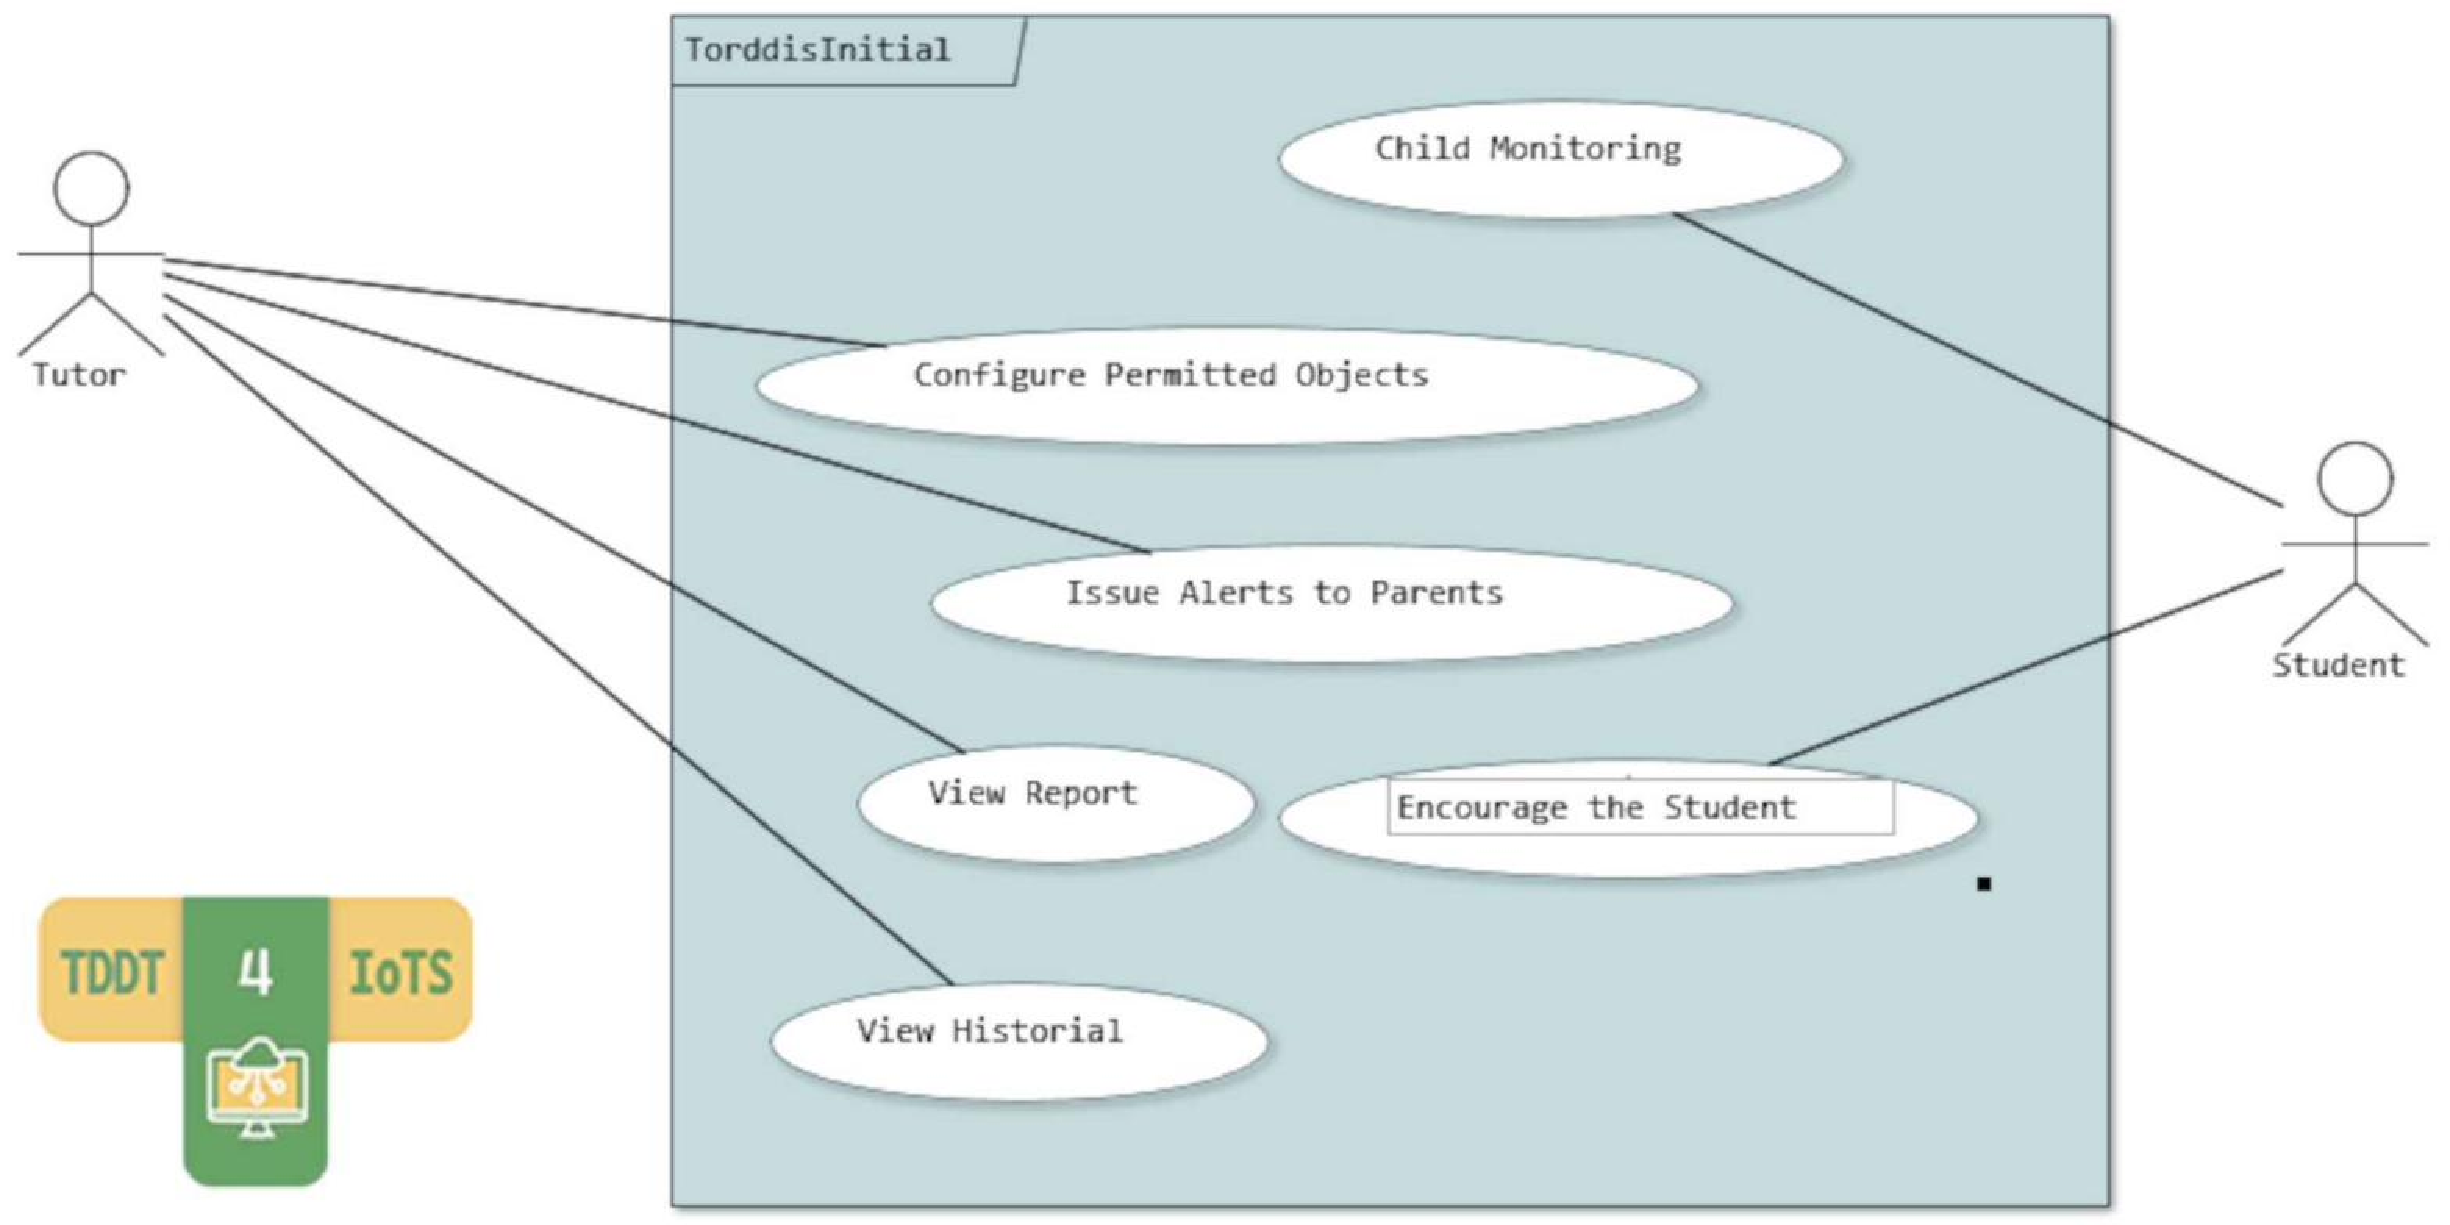
\includegraphics[frame,width=\linewidth]{Figure_2}
	\caption{High-level user requirements modelling of the Torddis system.\label{fig:UseCaseDiagram}}
\end{figure}

\subsection{Architecture and AI Modules}
The Torddis architecture was described following the framework established by \citet{ISO-IEC-IEEE42010-2022}, identifying three stakeholder groups (the \textit{guardian}, the \textit{monitored child} and the \textit{development team}) and their main concerns (in-session supervision, non-intrusiveness, data privacy and maintainability). Figure~\ref{fig:TorddisArchitecture} presents the deployment view, in which the IoT device on the child's desk streams video to an application server that hosts the four AI recognition modules and communicates with the guardian's mobile application over a secure channel.

\begin{figure}[!htbp]
	\centering
	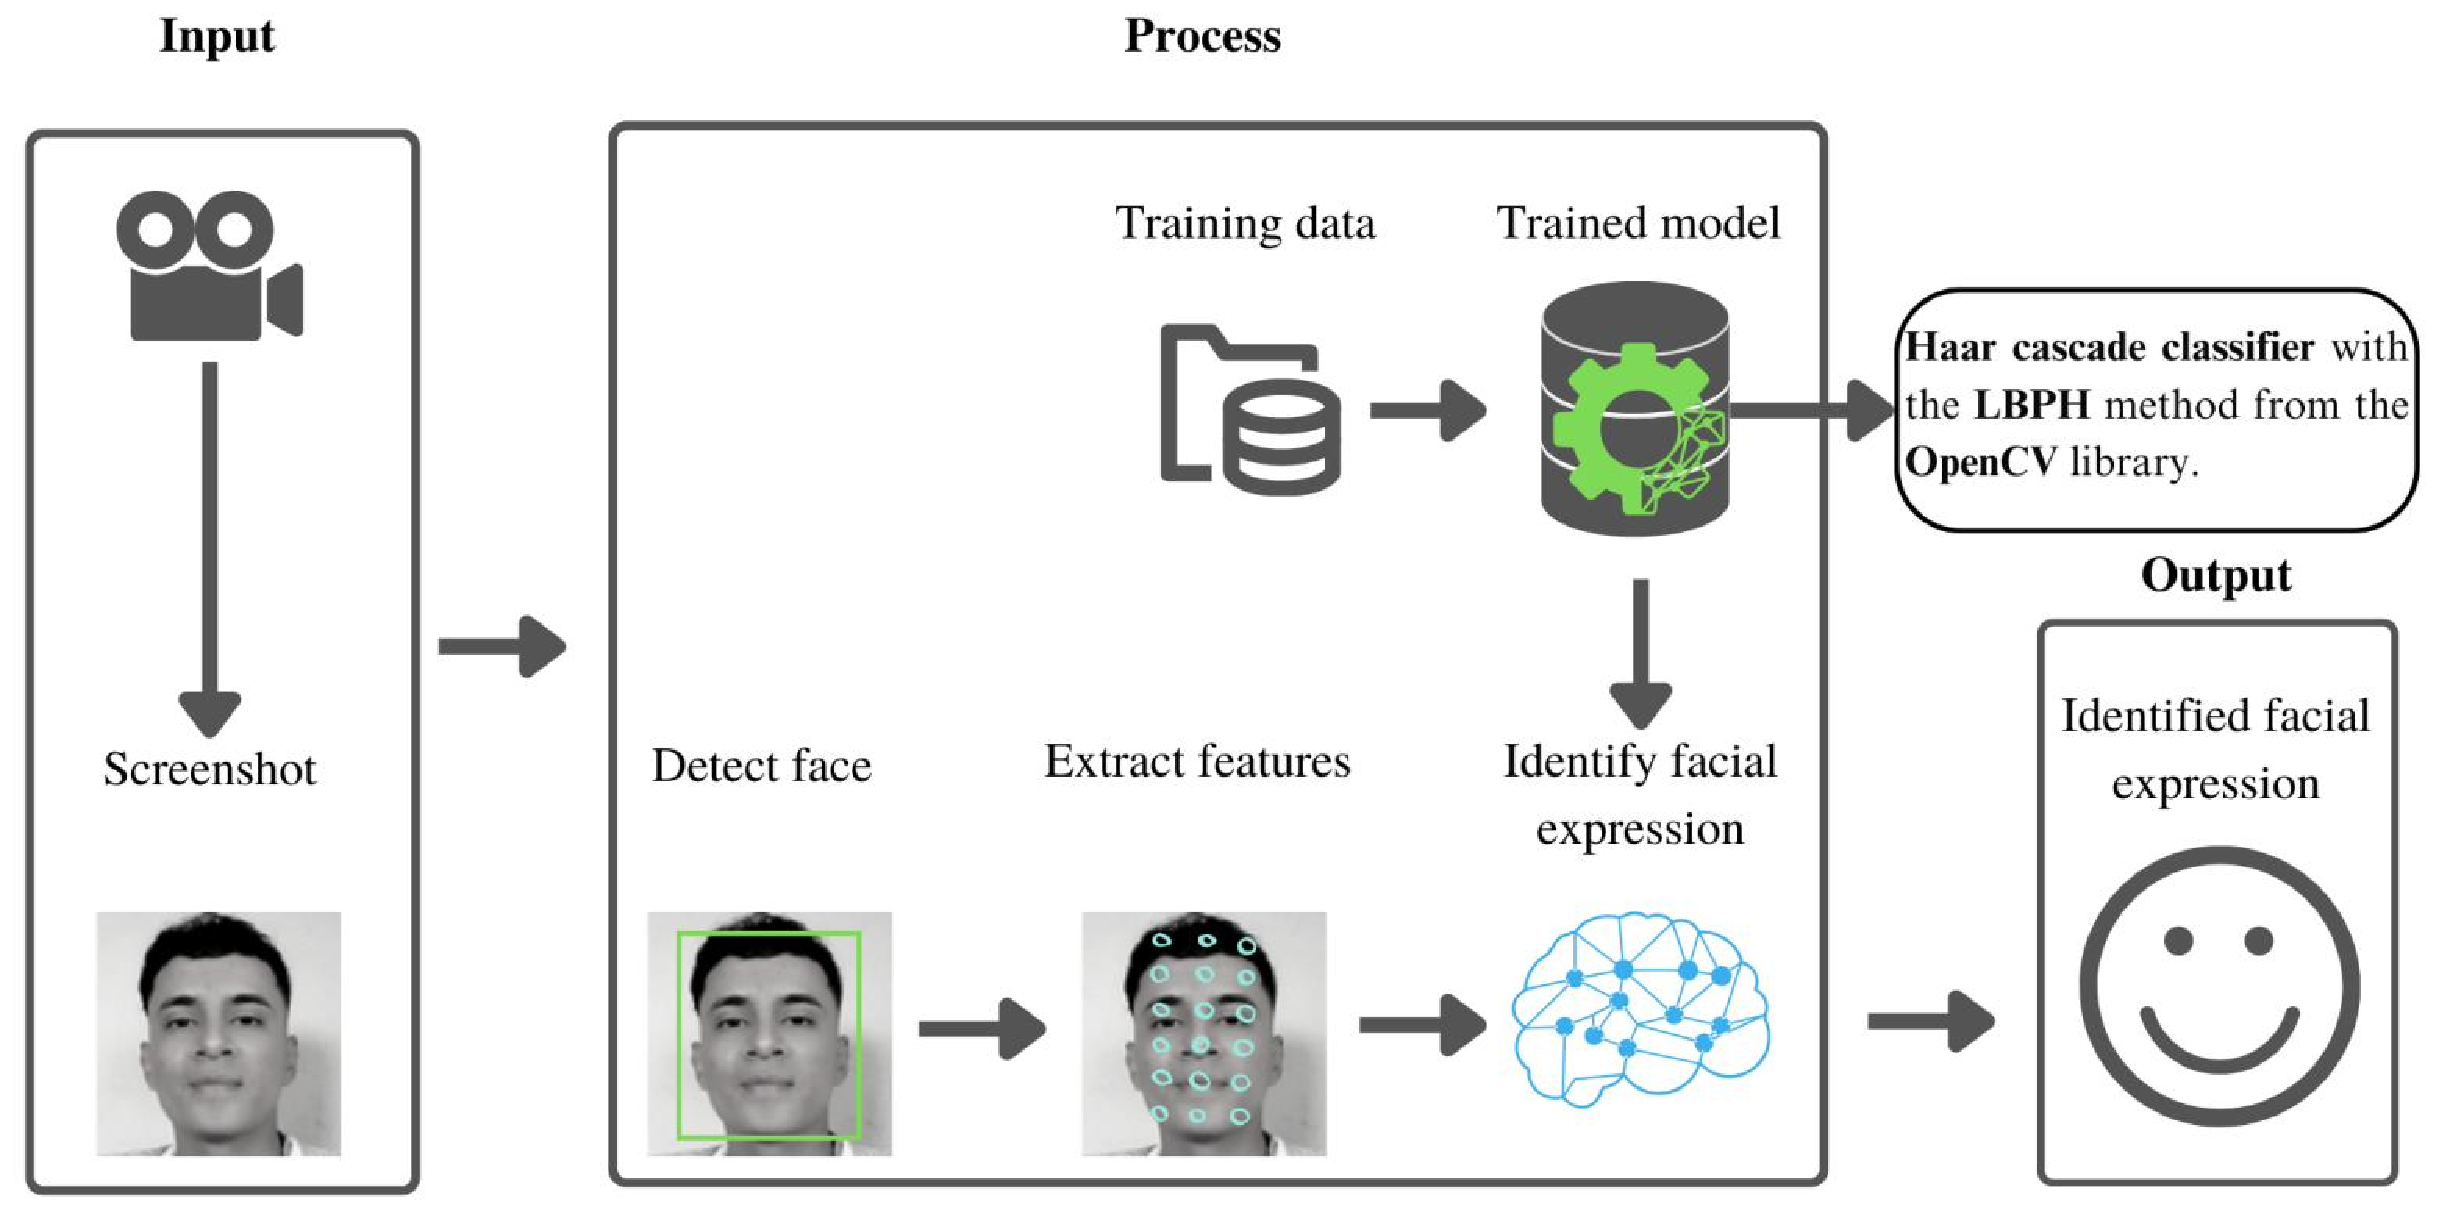
\includegraphics[frame,scale=0.5, width=0.9\linewidth]{Figure_3}
	\caption{Deployment diagram (nodes) of the Torddis system.\label{fig:TorddisArchitecture}}
\end{figure}

Figure~\ref{fig:TorddisDevice} shows the physical assembly of the IoT device, built around an ESP32-CAM module from Espressif Systems---which integrates an ESP32 SoC with an on-board OV2640 CMOS camera---and a NodeMCU~LoLin~V3 board based on the ESP8266 Wi-Fi microcontroller, which drives two alerting peripherals (a piezoelectric buzzer for auditory alerts and a red light-emitting diode for visual alerts) that are triggered whenever a distraction event is detected.

\begin{figure}[!htbp]
	\centering
	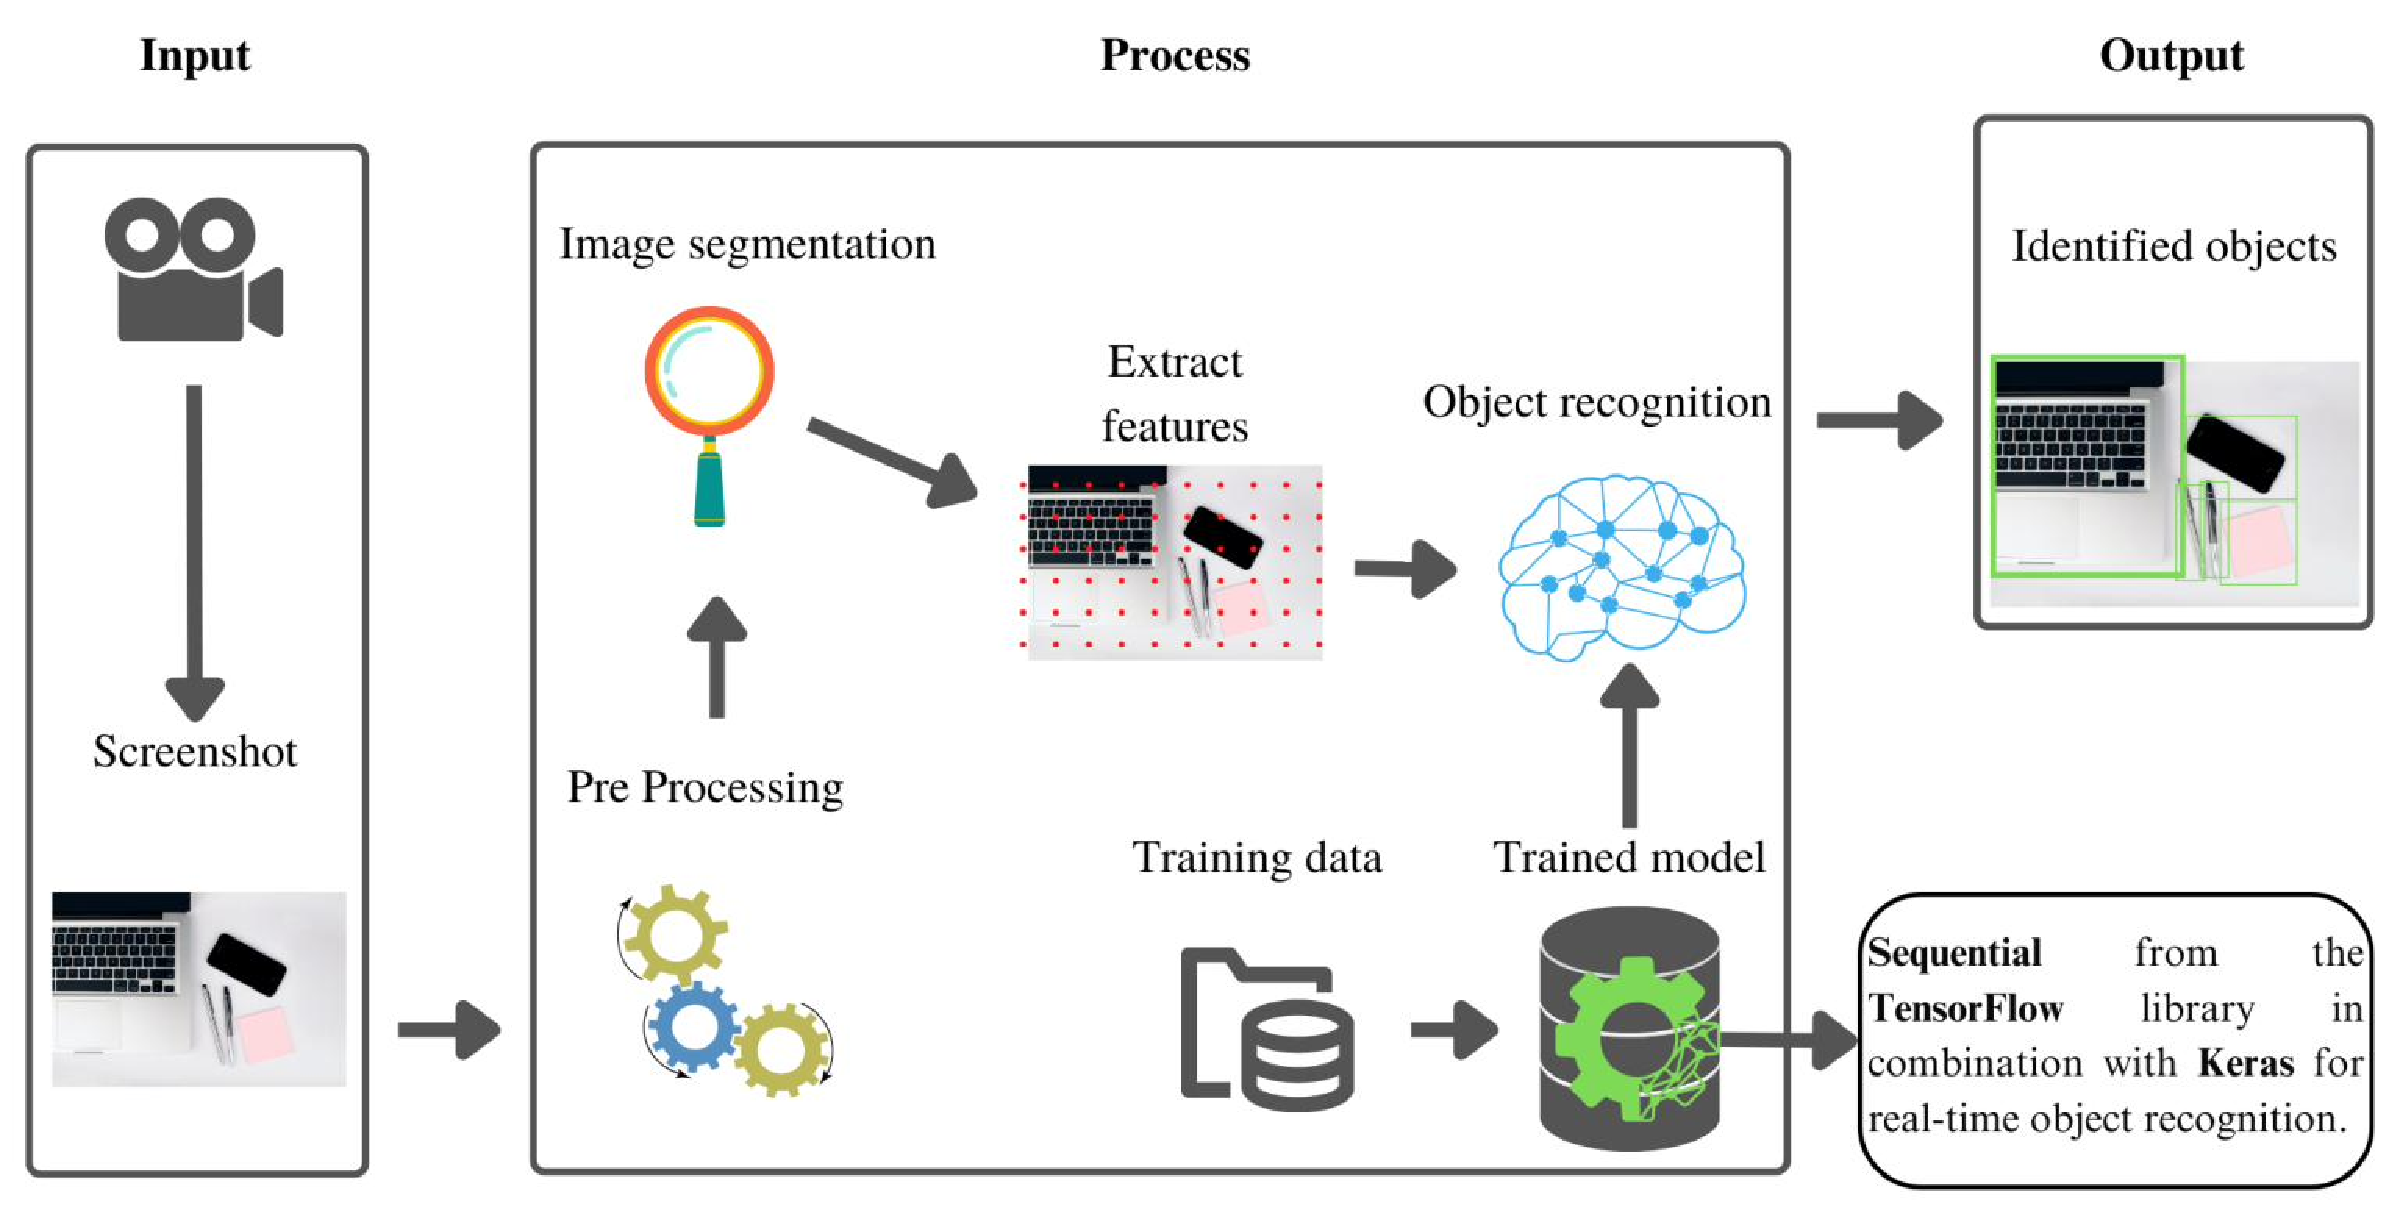
\includegraphics[frame,scale=0.5, width=0.78\linewidth]{Figure_4}
	\caption{Design of the IoT device of the Torddis system, showing its five main hardware components: (1)~ESP32-CAM module, (2)~NodeMCU~LoLin~V3 (ESP8266), (3)~solderless breadboard, (4)~piezoelectric buzzer, and (5)~red LED.\label{fig:TorddisDevice}}
\end{figure}

The recognition pipeline is implemented on the application server using established open-source libraries: a Convolutional Neural Network (CNN) for facial-expression recognition, a Haar cascade classifier with the Local Binary Pattern Histogram (LBPH) method from OpenCV for facial identity recognition, a Sequential model combined with TensorFlow and Keras for the detection of distractive objects, and Face Mesh from the MediaPipe library for drowsiness-state detection. These four modules operationalise the two classes of distraction identified during the detailed requirements analysis: \textit{internal distraction} (facial expressions associated with core emotions and drowsiness state) and \textit{external distraction} (presence of unfamiliar people, abandonment of the study area and the presence of objects that divert attention from the ongoing academic tasks) \citep{Asish2022Detecting,Vettivel2018System,Pabba2022AnIntelligent}. The comparative review of the AI methods evaluated for each recognition task is provided as Online Resource~2 (Supplementary Information, Section~S2), and Figure~\ref{fig:TorddisApp} shows the mobile application and the physical IoT device as delivered to the participating households.

\begin{figure}[!htbp]
	\centering
	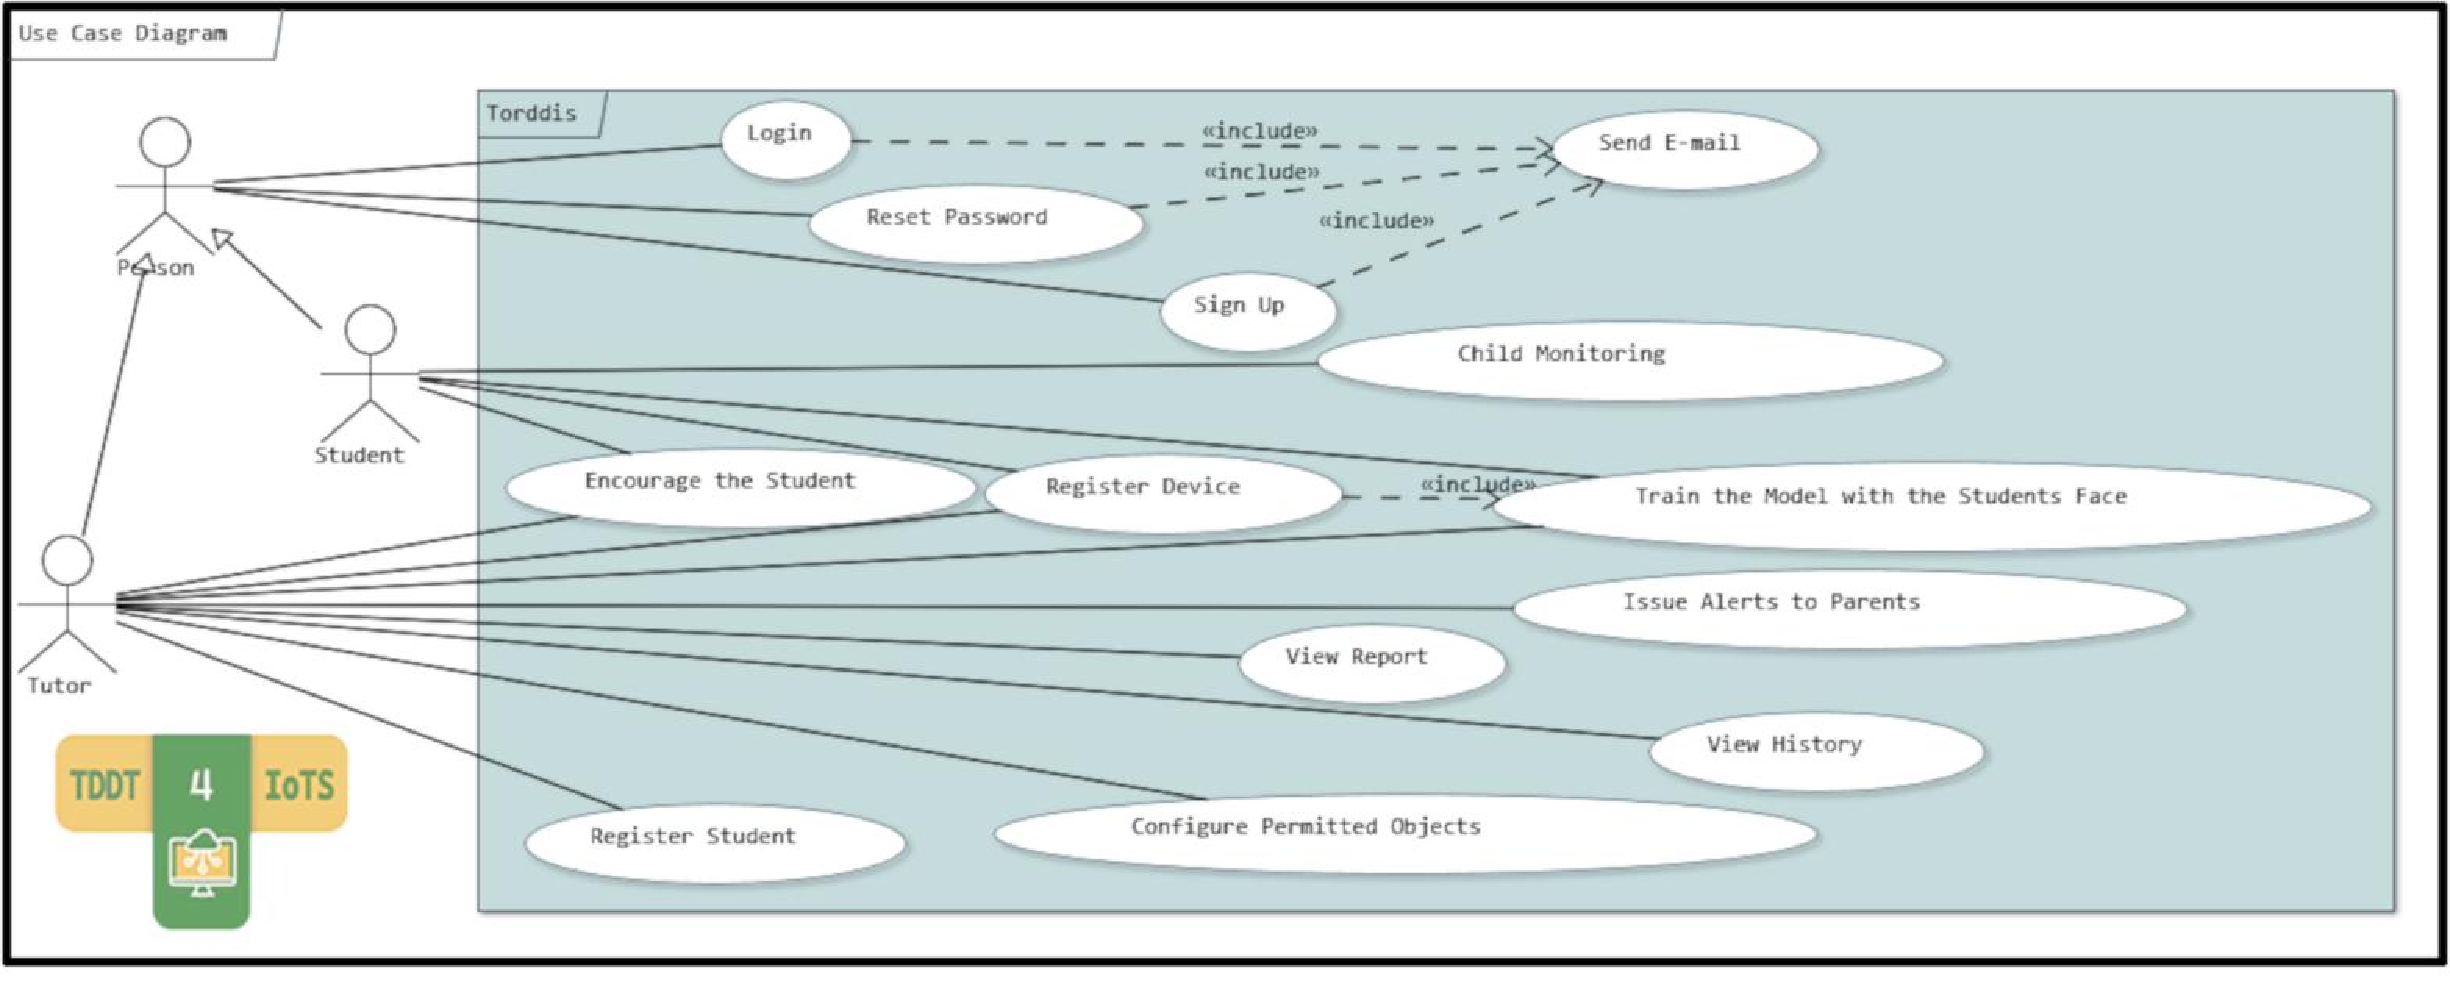
\includegraphics[width=\linewidth]{Figure_7}
	\caption{Screenshots of the mobile application and the Torddis IoT device.\label{fig:TorddisApp}}
\end{figure}

\subsection{Engineering Process at a Glance}
The engineering process followed TDDM4IoTS \citep{Guerrero-Ulloa2020TDDM4IoTS} and was supported end-to-end by the TDDT4IoTS tool \citep{Guerrero2024Test}, which generated the unit-test baseline and the code scaffolding from the semi-structured use-case specifications; the resulting 51-test suite---of which the 10 acceptance tests (PU-01 to PU-10) were executed with guardians during the pilot reported in Section~\ref{section:sixth}---was traced to the FR/NFR set through a requirements-to-tests traceability matrix. To keep the focus of this article on the pedagogical contribution, the full engineering detail (the eleven life-cycle phases, the fine-grained use-case and class diagrams, the complete test pyramid documented following \citet{ISO-IEC-IEEE29119-1-2022}, and the maintenance plan aligned with \citet{ISO-IEC-IEEE12207-2017}) is provided as Online Resource~2 (Supplementary Information, Sections~S3 and~S11).

\subsection{Standards Compliance and Ethical Considerations}
\label{ss:standards}
The Torddis life cycle was aligned with seven international standards covering software and system life-cycle processes \citep{ISO-IEC-IEEE12207-2017,ISO-IEC-IEEE15288-2023}, requirements engineering \citep{ISO-IEC-IEEE29148-2018}, product quality \citep{ISO-IEC25010-2023}, architecture description \citep{ISO-IEC-IEEE42010-2022}, software testing \citep{ISO-IEC-IEEE29119-1-2022} and information-security management \citep{ISO-IEC27001-2022}; the complete compliance-mapping table that lists the artefact(s) materialising conformance to each standard is provided as Online Resource~2 (Supplementary Information, Section~S6).

Because the study processed data relating to children, the protocol was reviewed and approved by the Research Committee of the Faculty of Engineering Sciences of the Universidad T\'ecnica Estatal de Quevedo (UTEQ), which is the competent oversight body for non-clinical educational-technology research at the host institution, since the university does not operate a clinical institutional review board with jurisdiction over studies of this nature; the study followed the principles of the Declaration of Helsinki and the data-protection provisions applicable in the participants' jurisdiction, aligned with \citet{ISO-IEC27001-2022}. Written informed consent was obtained from each parent or legal guardian on behalf of the child, and every participating child received an age-adapted, read-aloud assent script and gave verbal assent before each session, with both guardian and child free to stop the session at any moment without consequence; the blank consent and assent instruments are publicly available in the \texttt{ethics/} directory of the reproducibility repository.

The system was designed under a data-minimisation principle: no image, video or audio of the children is ever stored or published. The ESP32-CAM frames are processed in volatile memory for the duration of the inference (under 500~ms) and then immediately discarded, so that only derived events (presence, facial-expression category, drowsiness state and use of non-permitted objects), together with their time-stamps, are retained; consistently, the screenshots reproduced in this manuscript were captured with adult research staff rather than with participating children. Guardian data were pseudonymised at capture (identifiers G01--G12, with ages bucketed to five-year ranges), stored encrypted at rest (AES-256) and in transit (TLS~1.3 with certificate pinning), and accessed only through a named, audited list of authorised researchers; the identity-to-pseudonym mapping is held on paper under lock at the host institution and destroyed one year after publication of the manuscript.

A Privacy Impact Assessment following the framework of \citet{ISO-IEC27001-2022} (Annex~A) documented eight privacy risks---ranging from unauthorised access to raw frames to child anxiety induced by the alarm---together with their mitigations, reducing every residual risk to a \textit{low} or \textit{very low} level; in particular, the alarm escalates from a visual (LED) cue to a soft 500~ms auditory chime only after two consecutive events, so as not to startle the child. The complete Privacy Impact Assessment and the Data Management Plan are provided in the \texttt{ethics/} directory of the reproducibility repository.

\section{Methodological Design of the Study and Experimental Validation}
\label{section:fifth}
This study is based on a methodological approach that seeks to establish a bridge between technological design and pedagogical processes, with the aim of rigorously evaluating the impact of Torddis in real-world usage contexts. This section outlines the validation strategy employed, understood not only as a technical phase but as a key instance for articulating theory, user experience, and empirical evidence. The adopted methodological structure responds to both scientific validity requirements and the need to generate applicable knowledge in dynamic and diverse educational environments.

\subsection{Participants and Study Context}
The study involved 12 children and their respective guardians, selected through convenience sampling. The children, aged between 7 and 12 years, were enrolled in primary and lower secondary education. The guardians, aged between 25 and 65, had primary and secondary education levels. Participants resided in both urban and rural areas with access to basic services (electricity, drinking water, internet, and mobile telephony).

The selection criteria ensured that households had access to home internet (Wi-Fi or mobile data) and mobile data on the guardian’s smartphone, which were necessary conditions for system deployment. This approach ensures that the participants reflect the profile of potential Torddis users: families with guardians engaged in activities inside and outside the home, responsible for school-aged children requiring supervision.

The representativeness of the sample is considered acceptable given that real users of the system were involved and the defined inclusion criteria were met. Convenience sampling is appropriate for preliminary investigations such as this, allowing the collection of significant data despite limited availability or willingness of families to participate \citep{DiPietro2025Meta}.

\subsection{Experimental Process and Instrument Validation}
The experimental process was conducted in two phases, which are described in the following subsections.

\subsubsection{Controlled Environment}
This phase was designed to evaluate the system’s usability and performance. During the evaluation, guardians used the Torddis prototype with their children for 30 minutes in a previously prepared environment where all system functionalities were verified. To collect user experience data, SUS-type questionnaires and open-ended questions were administered.

\subsubsection{Real Environment}
This phase aimed to evaluate system effectiveness. It lasted one week, considering that only a single prototype was available. A Likert-scale questionnaire was used to assess guardians' perceptions of the system’s utility and effectiveness (reproduced in Online Resource~2, Section~S9.4), including questions on device attractiveness, notification accuracy, and its impact on children's self-regulation and concentration \citep{Ackermans2025Young}.

Instrument validity was ensured through expert review, confirming the clarity and relevance of the questions for the study’s purpose. In addition, system-generated data (e.g., detection of distracting objects and alerts) were manually verified to guarantee accuracy \citep{Wang2025Development}. The data were also analyzed to determine whether the variables followed a normal distribution, thereby guiding the choice of appropriate statistical methods (ANOVA, Kruskal–Wallis) and correlation coefficients (Pearson and Spearman).

\subsection{Randomization and Bias Control}
No randomization process was implemented due to the nature of the convenience sample. However, the following measures were adopted to minimize bias \citep{Huang2025How}:

\begin{itemize}
	\item Detailed explanation of each questionnaire item before participant completion.
	
	\item Assurance of anonymity and confidentiality of responses.
	
	\item Questionnaire administration without the presence of researchers to avoid influencing responses.
\end{itemize}

Nonetheless, three threats to validity are explicitly acknowledged. First, during the monitored sessions an evaluator (one of the authors) and one or both guardians remained in the room, approximately three metres from the child, so the \textit{independence condition} reflects passive adult presence---a simulated rather than a genuine absence of supervision---and the child's behaviour may not represent truly unsupervised study. Second, the presence of the evaluator together with the short one-week window make Hawthorne and novelty effects a plausible alternative explanation for the favourable perceptions, which may attenuate once the device is no longer a novelty. Third, the researchers' proximity to the participating families may have influenced their questionnaire responses \citep{DiPietro2025Meta}. These threats motivate the blinded, evaluator-absent and longer-term designs outlined in Section~\ref{section:eight}.

\subsection{Instruments and Statistical Analysis}
Four instruments were administered in addition to the demographic survey: (i)~the ten-item \textbf{System Usability Scale (SUS)} \citep{Brown1989}, preprocessed by reverse-scoring negatively worded items and rescaling from 0 to 100 for international comparability; (ii)~an eight-item open-ended questionnaire to elicit qualitative feedback on usability and effectiveness; (iii)~a seven-item Likert questionnaire validated by an expert panel for clarity and relevance, measuring guardians' perceptions of system effectiveness in the home setting (device attractiveness, non-intrusiveness, and perceived improvements in self-regulation and concentration); and (iv)~system-generated event metrics (frequency and duration of supervision, number of alerts issued and effective device usage time). The four instruments are reproduced in Online Resource~2, Section~S9. Data were subjected to descriptive statistics \citep{Yaska2024Assessment}, normality assessment via the Shapiro--Wilk \citep{Souza2023Sample} and Kolmogorov--Smirnov \citep{Lilliefors1969Kolmogorov} tests, Pearson \citep{Yu2024Inferential} and Spearman \citep{Yu2024Robust} correlation \citep{Jebb2021Review}, one-way ANOVA \citep{Dubey2025Two,Rojas2025Validating} with Post Hoc tests \citep{Ogrodniczek2025Comparative}, and the Kruskal--Wallis test \citep{Jamil2024Influence,Smeeton2025Applied}; the choice between parametric and non-parametric routes was driven by the Shapiro--Wilk outcome. Because the sample comprises only twelve guardian--child dyads, all inferential procedures are statistically underpowered and are therefore reported as exploratory, hypothesis-generating analyses, accompanied by effect-size estimates (the Pearson and Spearman correlation coefficients) and, for the Post Hoc comparisons, 95\% confidence intervals (Online Resource~2, Section~S4), and without correction for multiple comparisons. The full results of each of these analyses are reported in Section~\ref{sec:stats-analysis}.

\subsection{Limitations and Generalization}
The study has certain limitations:

\begin{enumerate}
	\item The sample was limited to a small group selected via convenience sampling, which may not represent other sociodemographic or technological contexts.
	
	\item The real-world phase lasted only one week, limiting the assessment of the system’s long-term impact on self-regulation skills.
	
	\item Only one prototype was available, restricting simultaneous use by multiple participants.
	
	\item With only twelve participants, the inferential analyses (ANOVA, Kruskal--Wallis, Pearson and Spearman) are statistically underpowered; they are consequently treated as exploratory and hypothesis-generating, are reported together with effect-size estimates and 95\% confidence intervals (Online Resource~2, Section~S4), and were not adjusted for multiple comparisons, so the associated significances are indicative rather than confirmatory.
	
	\item The primary effectiveness outcome, \textit{Statement (5)}, is a single-item, retrospective and guardian-reported proxy captured after one week; it was not triangulated with an objective or psychometrically validated measure of self-regulation or concentration, nor with the child's own report, which constrains the construct validity of the central finding and calls for multi-item, longitudinal and behaviourally-anchored measurement in future studies.
	
	\item The evaluation was neither blinded nor free of researcher presence: an evaluator and the guardians remained in the room during the monitored sessions and the deployment lasted only one week, so Hawthorne and novelty effects cannot be excluded as partial explanations of the favourable perceptions, and the \textit{independence condition} reflects passive adult presence rather than genuine unsupervised study.
	
	\item The study does not directly measure Zimmerman's self-regulated-learning subprocesses: the mapping in Table~\ref{tab:srl-mapping} is a theoretical design rationale, and the effectiveness questionnaire captures guardian-perceived global outcomes rather than phase-specific forethought, performance or self-reflection processes, so the pedagogical mapping remains to be empirically validated with instruments that operationalise those subprocesses.
\end{enumerate}

These limitations are common in pilot or early-stage studies exploring educational technology impact.

Previous studies have highlighted that the generalizability of results from technological interventions strongly depends on population characteristics and implementation context. For example, a recent meta-analysis on the effects of technology on disadvantaged students emphasizes how resource access and contextual conditions can significantly influence outcomes. It recommends designing future studies with broader and more diverse populations to enhance representativeness \citep{DiPietro2025Meta}. Cross-cultural evidence also indicates that the effect of extramural ICT factors on academic performance and well-being is moderated by the type of self-regulated learner---weaker self-regulated learners being particularly susceptible in East Asian samples and stronger self-regulated learners in Western samples \citep{Chen2024Extramural}. This heterogeneity motivates future stratification of Torddis outcomes by learner profile.

\subsection{Validation of the TDDM4IoTS Methodology}
TDDM4IoTS \citep{Guerrero-Ulloa2020TDDM4IoTS} was selected for its explicit focus on IoT projects and its capacity to enable iterative hardware--software integration with automated unit-test generation \citep{Guerrero-Ulloa2023Nawi,Guerrero2024Test}. Its application to Torddis provided a systematic mapping of requirements to test artefacts and to source-code scaffolding, aligning the life cycle with the standards listed in Section~\ref{ss:standards}, and offered the pedagogical benefit of coupling early technical validation with the iterative refinement that at-home educational technologies typically require to reach a domestic-ready form factor \citep{Borte2024Learning,Wang2025Development}.

\section{Results}
\label{section:sixth}
This section presents the empirical results of the Torddis pilot evaluation. Two dimensions are reported: (i)~the usability of the mobile application and IoT device, as perceived by the guardians who supervised its use at home, and (ii)~the technical performance of the AI recognition modules under real-world operating conditions. The complementary statistical analyses of the guardians' effectiveness questionnaire are presented in Subsection~\ref{sec:stats-analysis}.

\subsection{Deliverable Evaluation}
Each deliverable (mobile application and device) was evaluated by the user in an ideal setting. Figure~\ref{fig:ConfigEvaluation} shows the configuration of one of the environments used to evaluate the Torddis system. The child is seated at a desk performing school tasks while being monitored by the Torddis system.

\begin{figure}[!htbp]
	\centering
	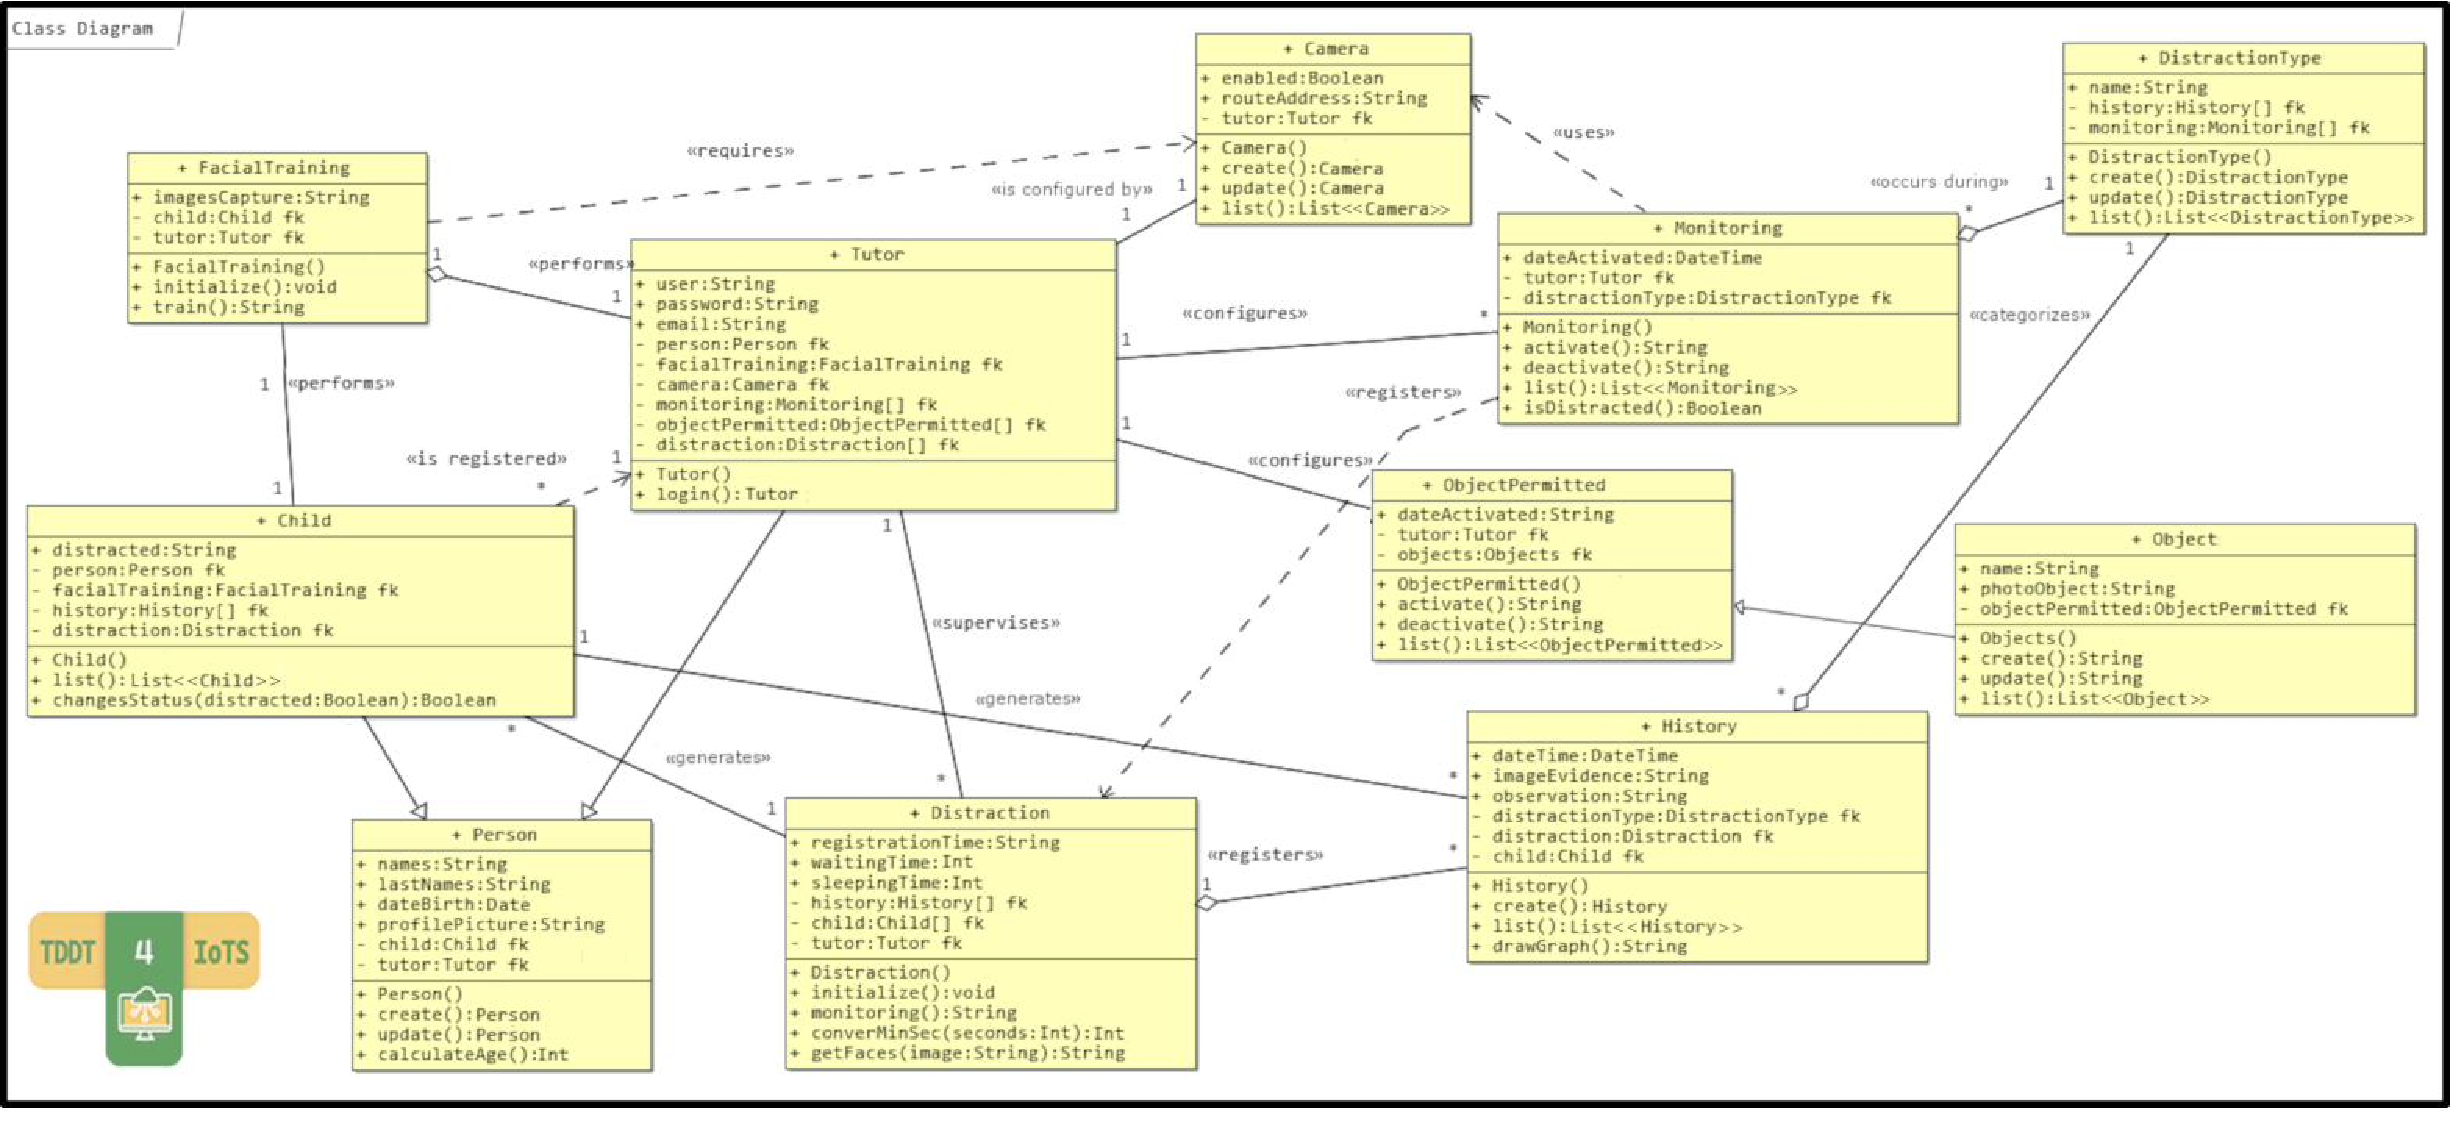
\includegraphics[width=\linewidth]{Figure_8}
	\caption{Setup of the environment for evaluating the Torddis system.\label{fig:ConfigEvaluation}} 
\end{figure}

The system is capable of monitoring the student’s concentration and identifying distractions. The device is placed at a distance of 50 to 70 cm from the child to ensure optimal camera operation, which provides the necessary input for facial recognition and object detection technologies. It is worth noting that, from the child’s perspective, the device is intended to be perceived as a decorative item on the desk.

An evaluator (one of the authors of this article), along with one or both parents, is present (seated in front of the TV). They are positioned approximately three meters from the child. The evaluator supervises the system’s operation via a laptop, while the parent(s) use the mobile application integrated with the IoT device to monitor the child’s concentration with low latency.

This setup allowed for a comprehensive evaluation of the Torddis system, ensuring that all involved parties (children, parents, and evaluators) could interact with the technology and provide valuable feedback on its effectiveness in monitoring and enhancing concentration during academic activities.

To evaluate the system's functionalities as a whole, five acceptance test cases were designed and executed, covering guardian account creation, login, facial training, device registration, and configuration of monitored objects. Their detailed specifications --- following the guidelines of \cite{Sciarra2024Smash} --- are provided as Online Resource~1 (Supplementary Information, Section~S1).

\subsubsection{Usability Evaluation of the Developed System Prototype}
The usability evaluation of the Torddis system was conducted to collect information about the overall user experience, focusing specifically on ease of use, interface design, and the effectiveness of the features provided. This comprehensive evaluation aimed to identify strengths and areas for improvement, ensuring that the system effectively meets user needs. The following subsections detail the demographic data of the participants, their experiences, the specific tasks performed during the evaluation, and the results obtained through the use of Likert-scale questionnaires (reproduced in Online Resource~2, Section~S9.2) and open-ended questions (reproduced in Online Resource~2, Section~S9.3) from the System Usability Scale (SUS) \citep{Brooke1996SUS}.

\noindent\textbf{Demographic Data.}
At the beginning of the usability evaluation of the Torddis system, a demographic questionnaire was provided (reproduced in Online Resource~2, Section~S9.1) to gather information about the guardians who participated in the evaluation. The sample size of 12 guardians was determined by three convergent criteria. First, this was a formative pilot deployment in real domestic settings whose primary aim was to obtain a reliable perceived-usability estimate under the System Usability Scale (SUS) and to elicit qualitative feedback for design iteration, rather than to test hypotheses at large scale; the SUS literature has repeatedly shown that samples of twelve to fourteen participants are sufficient to reach the same conclusion as substantially larger samples in at least 90\% of comparisons \citep{Orfanou2015Perceived}. Second, the requirement that each family provide seven consecutive days of at-home deployment---involving parental installation of the IoT device, daily supervision of the sessions and completion of two questionnaires---limited the pool to volunteer households prepared to commit that level of engagement. Third, the demographic composition explicitly sought variation in guardian gender, age, education level and area of residence (urban/rural) to ensure the sample was not homogeneous, at the cost of enlarging it beyond what a pilot warrants. The questionnaire yielded the following results:

\begin{itemize} 
	\item A total of 12 guardians were evaluated, represented by 8 mothers and 4 fathers, all from the geographic area of Quevedo, Ecuador.
	\item The average age of the participants was 39 years, ranging from 25 to 65 years.
	\item 58\% of the guardians had completed only primary education, while 42\% had reached secondary education.
\end{itemize}

\noindent\textbf{About Monitoring.}
Four preliminary questions were posed to characterise the baseline supervision context. Guardians rated the monitoring of distraction signs during homework as a complex task (7~of~12 selected ``complex'', 4 ``moderate'', 1 ``easy''), reported the need to supervise constantly (6 ``always'', 3 ``almost always'', 3 ``sometimes''), and cited verbal warnings, motivational advice and small rewards (candies, toys, trips to the park, favourite meals) as the main strategies used to keep their children focused. The corresponding bar-chart visualisations are provided as Online Resource~2 (Supplementary Information, Section~S7).

\noindent\textbf{Tasks Performed by Participating Guardians.}
The tasks performed by the guardians during the usability evaluation covered three phases. In the \emph{setup phase}, the guardian connected the Torddis IoT device to mains power, placed it on the child's desk, created a guardian account, logged into the mobile application, registered the child, and registered the device using the Media Access Control (MAC) address from its label. In the \emph{configuration phase}, the guardian performed facial training for the registered child and enabled or disabled the objects (distractors) to be monitored. In the \emph{monitoring phase}, the guardian assigned the child a task (colouring a mandala), activated distraction-parameter detection, left the child to work for six minutes with the adults present but passive---a \textit{simulated-independence} condition rather than a genuine absence of supervision---enabled or disabled video streaming, and finally browsed the event history and viewed the graphical report of the detected distraction parameters.

\noindent\textbf{System Usability Scale (SUS) Questionnaire Results.}
The results analysed in this section correspond to the responses to the SUS questionnaire (reproduced in Online Resource~2, Section~S9.2) provided by the 12 guardians. Based on the collected data, Figure~\ref{fig:sus-questionnaire} shows a mean SUS score of 81.46 out of 100, with a standard deviation of 11.65. According to the adjective ratings (Worst imaginable, Poor, Acceptable, Good, Excellent, Best imaginable) proposed by \cite{Bangor2008AnEmpirical} to qualitatively interpret system usability scores, it is evident that Torddis achieved a “Good” level of usability based on the guardians’ evaluations.

\begin{figure}[!htbp]
	\centering
	\begin{tikzpicture}
		\begin{axis}[
			scatter/classes={
				a={mark=*,blue}
			},
			width=0.95\linewidth,
			height=8cm,
			xlabel={Participant},
			ylabel={Evaluation Score},
			ymin=40, ymax=100,
			xmin=0, xmax=13,
			xtick={1,2,3,4,5,6,7,8,9,10,11,12},
			xticklabels={1,2,3,4,5,6,7,8,9,10,11,12},
			ytick={40,60,80,100},
			nodes near coords,
			every node near coord/.append style={font=\footnotesize, /pgf/number format/fixed},
			legend style={at={(0.5,-0.15)}, anchor=north, legend columns=-1},
			enlarge x limits=0.05,
			]
			\addplot[
			scatter,
			only marks,
			scatter src=explicit symbolic,
			visualization depends on=\thisrow{Evaluation} \as \label
			] table[meta=class,x=Participant,y=Evaluation] {
				Participant Evaluation class
				1 90.00 90.00
				2 95.00 95.00
				3 72.50 72.50
				4 60.00 60.00
				5 85.00 85.00
				6 67.50 67.50
				7 92.50 92.50
				8 67.50 67.50
				9 82.50 82.50
				10 85.00 85.00
				11 92.50 92.50
				12 87.50 87.50
			};
			
			% Average line
			\addplot [
			color=orange,
			thick,
			mark=none
			] coordinates {(0,\average) (13,\average)};
			
			% Upper standard deviation
			\addplot [
			color=orange,
			thick,
			dashed,
			mark=none
			] coordinates {(0,\upperlimit) (13,\upperlimit)};
			
			% Lower standard deviation
			\addplot [
			color=orange,
			thick,
			dashed,
			mark=none
			] coordinates {(0,\lowerlimit) (13,\lowerlimit)};
			
			\legend{Participant, Mean SUS Score, Std. Deviation}
		\end{axis}
	\end{tikzpicture}
	\caption{Mean and standard deviation of guardians' responses to the SUS questionnaire.}
	\label{fig:sus-questionnaire}
\end{figure}

The results of the SUS questionnaire \citep{Brooke1996SUS} reflect a positive perception of the system, with scores emphasizing its ease of use and effectiveness. The consistency in users' responses demonstrates that the interface design and the initial setup processes are properly optimized for users with varying levels of technological experience. This reinforces the reliability of the system as an accessible tool for guardians with different educational backgrounds \citep{Deng2024Does}.

\noindent\textbf{Results of the Open-Ended Questions Questionnaire.}
At the end of the SUS questionnaire, the guardians answered eight open-ended questions (reproduced in Online Resource~2, Section~S9.3) to elicit personal opinions on the Torddis prototype. Questions~1, 2, 6 and 8 admitted categorical response coding, whose distribution across the 12 guardians is summarised in Table~\ref{tab:open-answers-summary}; the corresponding bar-chart visualisations are provided as Online Resource~2 (Supplementary Information, Section~S7).

\begin{table}[!htbp]
	\centering
	\caption{Frequency of response categories to the four categorical open-ended questions.}
	\label{tab:open-answers-summary}
	\setlength{\tabcolsep}{5pt}
	\begin{tabular*}{\linewidth}{@{\extracolsep{\fill}}
			>{\raggedright\arraybackslash}p{5.8cm}
			>{\raggedright\arraybackslash}p{5.2cm}
			>{\centering\arraybackslash}p{1.6cm}
			@{}}
		\toprule
		\textbf{Open-ended question} & \textbf{Response category} & \textbf{Count} \\
		\midrule
		Q1. General opinion about the system & Supports concentration & 4 \\
		& Appealing design & 8 \\
		\midrule
		Q2. Auditory and visual alerts & Helps the student & 7 \\
		& Satisfaction & 5 \\
		\midrule
		Q6. Suggestions for improvement & Camera quality & 4 \\
		& Camera-mount support & 2 \\
		& No further improvements needed & 6 \\
		\midrule
		Q8. Reasons to recommend the system & Monitoring function & 7 \\
		& Appealing design & 5 \\
		\bottomrule
	\end{tabular*}
\end{table}

The remaining four open-ended items received qualitatively favourable feedback across all 12 guardians. Question~3 (design of the mobile application) elicited positive assessments of the graphical interface; Question~4 (data-visualisation appropriateness) elicited approval of the organisation of the event history and graphical reports; Question~5 (perceived pedagogical impact) confirmed that the prototype effectively supports children's concentration by keeping the guardian informed when distractions occur; and Question~7 (willingness to continue) confirmed that all guardians would continue to use Torddis. Question~1 (general opinion) yielded two coded categories, with 8 of 12 guardians highlighting the appealing design and the remaining 4 emphasising the system's contribution to concentration. Question~2 (auditory and visual alerts) revealed that 7 guardians believed the light alerts help keep the student awake, and 5 expressed satisfaction with the auditory alarms. Question~6 (potential improvements) collected suggestions to use a higher-quality camera and enhance the camera mounting support, although 6 of 12 guardians indicated that no further improvements were necessary. Question~8 (reasons to recommend the system) highlighted its usefulness in monitoring (7 guardians) and its appealing design (5 guardians).

\subsubsection{Recognition Analysis}
The pilot comprised 14 test sessions per recognition module. For each session, both a binary recognition-success flag and, where recognition succeeded, the latency (in seconds) were recorded. Two complementary performance indicators are therefore reported: the recognition success rate (the proportion of sessions in which the module correctly identified the target element) and the recognition latency, computed over successful sessions because a latency is only defined when recognition occurs. Across the 14 sessions, the recognition success rates were 92.9\% (13/14) for person recognition, 92.9\% (13/14) for facial-expression recognition, 85.7\% (12/14) for drowsiness detection and 78.6\% (11/14) for distractive-object identification, giving an overall success rate of 87.5\% (49/56); the corresponding failures (person: 1; facial-expression: 1; drowsiness: 2; distractive-object: 3) are retained and reported rather than discarded, and are summarised in Table~\ref{tab:recognition-performance}. The mean latencies over successful sessions were 0.812~s (SD~=~0.227) for person recognition, 1.284~s (SD~=~0.440) for facial-expression recognition, 3.433~s (SD~=~0.905) for drowsiness detection and 2.329~s (SD~=~0.791) for distractive-object identification; the two modules with an explicit NFR-05 latency target meet it---person recognition below 1.5~s and drowsiness detection below 5~s---while facial-expression and distractive-object recognition also operate below 5~s, and the tightest distribution is observed for person recognition (0.530--1.200~s). Because the success flag captures correct detections but not false positives, these figures are recognition (detection) rates rather than a full precision--recall characterisation; a confusion-matrix evaluation against an independently labelled ground truth---including false-positive alerts, which are pedagogically costly because they interrupt on-task behaviour---is left for future work. The full per-session table (success flags and latencies), the complete descriptive statistics for each module and the Pearson correlation matrix between module latencies are provided as Online Resource~2 (Supplementary Information, Section~S4).

\begin{table}[!htbp]
	\centering
	\caption{Recognition performance of the four AI modules over the 14 controlled sessions: success rate and mean latency (computed over successful sessions).}
	\label{tab:recognition-performance}
	\setlength{\tabcolsep}{5pt}
	\begin{tabular*}{\linewidth}{@{\extracolsep{\fill}}
			>{\raggedright\arraybackslash}p{4.4cm}
			>{\raggedleft\arraybackslash}p{1.8cm}<{\hspace*{6pt}}
			>{\raggedleft\arraybackslash}p{1.2cm}<{\hspace*{6pt}}
			>{\raggedleft\arraybackslash}p{1.9cm}<{\hspace*{6pt}}
			>{\raggedleft\arraybackslash}p{2.6cm}
			@{}}
		\toprule
		\textbf{Recognition module} & \textbf{Success/Total} & \textbf{Fail} & \textbf{Success rate} & \textbf{Mean latency (SD), s} \\
		\midrule
		Person recognition            & 13/14 & 1 & 92.9\% & 0.812 (0.227) \\
		Facial-expression recognition & 13/14 & 1 & 92.9\% & 1.284 (0.440) \\
		Drowsiness detection          & 12/14 & 2 & 85.7\% & 3.433 (0.905) \\
		Distractive-object detection  & 11/14 & 3 & 78.6\% & 2.329 (0.791) \\
		\midrule
		Overall                       & 49/56 & 7 & 87.5\% & --- \\
		\bottomrule
	\end{tabular*}
\end{table}

\subsection{Statistical Analysis of Guardians' Responses}
\label{sec:stats-analysis}

Because the pilot involved only twelve guardian--child dyads, the statistical analysis of the guardians' responses is framed as exploratory and hypothesis-generating rather than confirmatory: its purpose is to describe patterns and to generate hypotheses for subsequent larger studies, not to establish the effectiveness of Torddis.

Accordingly, descriptive statistics are prioritised, the inferential tests (ANOVA, Kruskal--Wallis, Pearson and Spearman) are reported together with effect-size estimates (the correlation coefficients) and, for the Post Hoc comparisons, 95\% confidence intervals (Online Resource~2, Section~S4), and no correction for multiple comparisons is applied, so that every reported significance is read as an indicative signal whose value lies in its magnitude and in its consistency across the parametric and non-parametric routes rather than in crossing a fixed threshold.

\subsubsection{Descriptive Statistics}
This section presents and analyzes the descriptive statistics obtained from the collected data. These statistics play a crucial role in understanding the behavior of the evaluated variables and their impact on the acceptance and effectiveness of the system.

Table \ref{table:DescriptiveStatistics} shows measures of central tendency, such as the mean and median, which allow for the identification of general patterns among guardians and students regarding the Torddis system. For instance, the average daily time devoted by guardians to supervising school tasks is approximately 2 hours, indicating active but limited participation due to their time constraints caused by everyday responsibilities. The responses to the statements related to the perception and use of the device (Statements (1) to (7), reproduced in Online Resource~2, Section~S9.4) reveal consistently high average values (ranging from 2.67 to 4.42 on a 5-point Likert scale), suggesting a general acceptance of the system. The seven-item effectiveness scale showed a high internal consistency (Cronbach's $\alpha = 0.94$; mean inter-item correlation $\bar{r} = 0.72$); however, a value this high---together with the fact that Statements~(6) and~(7) elicited identical responses from all twelve guardians ($r = 1.000$)---points to item redundancy rather than to a well-differentiated scale, so these items are interpreted as a single convergent indicator and their consolidation is recommended for future versions (see Section~\ref{sec:stats-analysis}).

\begin{table}[!htbp]
	\centering
	\caption{Descriptive statistics on supervision time and the usage and effectiveness of the developed device.}
	\setlength{\tabcolsep}{3pt}\begin{tabular*}{\linewidth}{@{\extracolsep{\fill}}>{\raggedright\arraybackslash}p{2.6cm} *{8}{>{\raggedleft\arraybackslash}p{0.85cm}<{\hspace*{3pt}}}@{}}
		\toprule
		\multicolumn{1}{c}{\textbf{Statistic}} & \multicolumn{1}{c}{\textbf{\shortstack{Superv.\\Time}}} & \multicolumn{1}{c}{\textbf{(1)}} & \multicolumn{1}{c}{\textbf{(2)}} & \multicolumn{1}{c}{\textbf{(3)}} & \multicolumn{1}{c}{\textbf{(4)}} & \multicolumn{1}{c}{\textbf{(5)}} & \multicolumn{1}{c}{\textbf{(6)}} & \multicolumn{1}{c}{\textbf{(7)}} \\
		\midrule
		Mean & 1.92 & 4.42 & 4.33 & 2.67 & 3.50 & 4.00 & 4.42 & 4.42 \\
		Median & 2.00 & 5.00 & 4.00 & 3.00 & 4.00 & 4.00 & 5.00 & 5.00 \\
		Standard Deviation & 0.67 & 0.79 & 0.65 & 0.99 & 0.91 & 0.74 & 0.79 & 0.79 \\
		Minimum & 1.00 & 3.00 & 3.00 & 1.00 & 2.00 & 3.00 & 3.00 & 3.00 \\
		Maximum & 3.00 & 5.00 & 5.00 & 4.00 & 5.00 & 5.00 & 5.00 & 5.00 \\
		\bottomrule
	\end{tabular*}
	\label{table:DescriptiveStatistics}
	\vspace{0.3em} % Space between table and note
	\parbox{0.85\textwidth}{\footnotesize
		Items (n) with $n=1\ldots7$ correspond to the seven statements evaluated on a 5-point Likert scale related to the prototype's effectiveness (reproduced in Online Resource~2, Section~S9.4). \textit{Supervision time} represents the number of daily hours that guardians dedicate to supervising their children's schoolwork.
	}
\end{table}

On the other hand, dispersion indicators, such as the standard deviation, provide insight into the variability of the responses. The standard deviation for the statements (ranging from 0.65 to 0.99) indicates that participants' perceptions were relatively homogeneous, which reinforces the consistency in the user experience of the device. However, the greater variability in \textit{Statement (3)} suggests that some students may have perceived the device as more intrusive, which could necessitate design adjustments.

Likewise, the minimum and maximum values reveal possible differences in participants’ experiences, highlighting areas that may require improvement. For instance, while some guardians reported dedicating only one hour to supervision, others reached up to three hours, which could influence the responses related to the system’s effectiveness.

These results make it possible to identify both the general level of acceptance of the system and specific areas that could benefit from targeted future interventions. Taken together, the descriptive statistics provide a foundation for validating the device’s design and supporting the discussion regarding its pedagogical and practical potential.

\subsubsection{Normality Analysis of the Data}
To determine whether the numerical variables follow a normal distribution, two complementary tests were applied: the Shapiro--Wilk (SW) test---sensitive to deviations from normality and particularly suitable for small samples \citep{Correa2025Simulation}---and the Kolmogorov--Smirnov (KS) test---more robust in the presence of heterogeneous variance \citep{Kobayashi2025Testing}. Both were reported jointly to obtain a complementary reading of the assumption.

Under the KS criterion all ten variables were compatible with normality ($p>0.05$). Under the more stringent SW criterion, three variables were compatible with normality (\textit{Guardian's Age}, $p=0.2277$; \textit{Student's Age}, $p=0.1736$; \textit{Statement~(3)}, $p=0.0528$; \textit{Statement~(4)}, $p=0.0598$), whereas six variables departed from normality ($p<0.05$): \textit{Supervision Time}, \textit{Statement~(1)}, \textit{Statement~(2)}, \textit{Statement~(5)}, \textit{Statement~(6)} and \textit{Statement~(7)}. The full per-variable table of SW and KS p-values is provided as Online Resource~2 (Supplementary Information, Section~S8). To ensure the validity of subsequent analyses, parametric tests (ANOVA, Pearson correlation) were applied to variables consistent with normality, and non-parametric tests (Kruskal--Wallis, Spearman correlation) were applied to those that departed from it under the SW criterion.

\subsubsection{Correlation between Statement (5) and the Other Variables}
Pearson correlation tests were used to explore associations among the variables under study. Before interpreting them, it must be made explicit that \textit{Statement (5)}---\textit{``After discontinuing use of the device, the student demonstrated improvement in self-regulation and concentration while completing homework at home''}---is a single-item, retrospective judgment reported by the guardian after one week of use; it is therefore a \emph{perceived} proxy for self-regulation and concentration, not an objective or psychometrically validated measure of either construct, and the associations reported below must be read in that light. With this caveat, and treating the variables flagged as normal, the analysis identified the associations between \textit{Statement (5)} and the remaining numerical variables shown in Table~\ref{table:Pearson-Correlation}.

\begin{table}[!htbp]
	\centering
	\caption{Correlations between Statement (5) and the Other Variables}
	\begin{tabular*}{\linewidth}{@{\extracolsep{\fill}}
			>{\raggedright\arraybackslash}p{4cm}
			>{\raggedleft\arraybackslash}p{3cm}<{\hspace*{8pt}}
			>{\raggedleft\arraybackslash}p{2cm}<{\hspace*{8pt}}
			>{\centering\arraybackslash}p{2.8cm}
			@{}}
		\toprule
		\multicolumn{1}{c}{\textbf{Variable}} & \multicolumn{1}{c}{\textbf{\shortstack{Correlation with\\Statement (5)}}} & \multicolumn{1}{c}{\textbf{\textit{p}-value}} & \multicolumn{1}{c}{\textbf{\shortstack{Type of\\Relationship}}} \\
		\midrule
		Age of the guardian$^{sw}$ & -0.2725 & 0.3916 & \(\bigtriangleup\) \\ % Weak
		Supervision time & 0.1841 & 0.5668 & \(\bigtriangleup\) \\ % Weak
		Age of the student$^{sw}$ & -0.1407 & 0.6627 & \(\bigtriangleup\) \\ % Weak
		Statement (1) & 0.7762 & 0.0030 & \(\bigstar\) \\ % Very Strong
		Statement (2) & 0.5669 & 0.0546 & \(\checkmark\) \\ % Strong
		Statement (3)$^{sw}$ & 0.7500 & 0.0050 & \(\bigstar\) \\ % Very Strong
		Statement (4)$^{sw}$ & 0.8165 & 0.0012 & \(\bigstar\) \\ % Very Strong
		Statement (6) & 0.7762 & 0.0030 & \(\bigstar\) \\ % Very Strong
		Statement (7) & 0.7762 & 0.0030 & \(\bigstar\) \\ % Very Strong
		\bottomrule
	\end{tabular*}
	\label{table:Pearson-Correlation}
	\vspace{0.3em} % Space between the table and the footnote
	\parbox{0.75\textwidth}{\footnotesize
		$^{sw}$ Normal variables according to the Shapiro-Wilk test.\\
		\(\bigtriangleup\): Weak. \(\checkmark\): Strong. \(\bigstar\): Very Strong.\\
		Statements~(6) and~(7) elicited identical responses (\(r=1.000\)); Statement~(1) is strongly collinear and coincidentally shares the same coefficient (\(r=0.7762\)) here. They are treated as one convergent dimension (see Section~\ref{sec:stats-analysis}).
	}
\end{table}

Firstly, the variables associated with the following statements—\textbf{Statement (1)}: \textit{The device was perceived by the student as appealing}, \textbf{Statement (3)}: \textit{The student did not perceive the presence of the device as intrusive}, \textbf{Statement (4)}: \textit{The device was used throughout the effective time devoted to performing school tasks}, \textbf{Statement (6)}: \textit{Although the device usage time was short, it is expected to significantly contribute to task completion and the academic performance of the student}, and \textbf{Statement (7)}: \textit{You would be willing to continue using the device}—showed \textit{very strong} positive correlations with \textit{Statement (5)}, with values ranging from 0.7500 to 0.8165. Also, \textbf{Statement (2)}: \textit{The mobile application accurately recorded the events that occurred}, yielded a strong correlation with \textit{Statement (5)} (\(r=0.5669\), \(p=0.0546\)).

It must be stressed that the coefficients of Statements~(1), (6) and~(7) coincide (\(r=0.7762\), \(p=0.0030\)), and that the same coincidence recurs in the ANOVA (\(F=11.0625\), \(p=0.0038\)). This does not constitute three independent effects: Statements~(6) and~(7) elicited \emph{identical} responses from all twelve guardians (\(r=1.000\)), so they are statistically the same variable, whereas Statement~(1) is strongly collinear with them (\(r=0.86\)) and coincides in these particular statistics only by chance in such a small sample. Accordingly, Statements~(1), (6) and~(7) are read as convergent indicators of a single underlying dimension---overall acceptance of, and willingness to keep using, the device---rather than as separate corroborations, consistent with the exploratory framing of this section and with the high internal consistency reported above (Cronbach's \(\alpha=0.94\)).

Although age is often regarded as an indicator of greater responsibility \citep{Moss2018Why}, in this study, the variables \textit{Age of the guardian} and \textit{Age of the student} exhibited weak and non-significant correlations, with values of \textbf{-0.2725} and \textbf{-0.1407}, respectively. These findings suggest that the perceived effectiveness of the device is not influenced by the age of either guardians or students. This result highlights the versatility of the system, demonstrating its applicability across diverse demographic groups without being constrained by age-related factors.

Finally, within this small exploratory sample the results are consistent with the interpretation that characteristics directly related to device usage---such as its design and operational effectiveness---are more strongly associated with perceived self-regulation than demographic factors. This pattern is offered as a hypothesis about the value of user-centred design in technology-based educational systems, to be tested in larger confirmatory studies, rather than as strong evidence.

\subsubsection{ANOVA Analysis}
As an exploratory check on whether responses to \textit{Statement (5)} co-vary with the remaining items, a one-way ANOVA was computed for each variable; with only twelve observations these tests are underpowered, so the results in Table~\ref{table:ANOVA-Results} are read as indicative patterns rather than as evidence of the system's impact. Several statements linked to the perceived effectiveness of the device differed at the conventional $\alpha = 0.05$ level, while the demographic variables did not; because no correction for multiple comparisons was applied and the sample is small, these p-values are interpreted as indicative signals rather than as confirmatory findings.

\begin{table}[!htbp]
	\centering
	\caption{ANOVA analysis results}
	\begin{tabular*}{\linewidth}{@{\extracolsep{\fill}}
			>{\raggedright\arraybackslash}p{4.5cm}
			>{\raggedleft\arraybackslash}p{2.5cm}<{\hspace*{8pt}}
			>{\raggedleft\arraybackslash}p{2.5cm}<{\hspace*{8pt}}
			>{\centering\arraybackslash}p{2.5cm}
			@{}}
		\toprule
		\multicolumn{1}{c}{\textbf{Variable}} & \multicolumn{1}{c}{\textbf{\textit{F}-Statistic}} & \multicolumn{1}{c}{\textbf{\textit{p}-value}} & \multicolumn{1}{c}{\textbf{Conclusion}} \\
		\midrule
		Guardian's Age$^{sw}$ & 0.8162 & 0.4723 & \(\times\) \\ % No significant differences
		Supervision Time & 0.2411 & 0.7907 & \(\times\) \\ % No significant differences
		Student's Age$^{sw}$ & 1.6419 & 0.2467 & \(\times\) \\ % No significant differences
		Statement (1) & 11.0625 & 0.0038 & \(\bigstar\) \\ % Highly significant difference
		Statement (2) & 2.9118 & 0.1059 & \textit{NS} \\ % Not significant
		Statement (3)$^{sw}$ & 5.7857 & 0.0242 & \(\checkmark\) \\ % Significant difference
		Statement (4)$^{sw}$ & 10.6875 & 0.0042 & \(\bigstar\) \\ % Highly significant difference
		Statement (6) & 11.0625 & 0.0038 & \(\bigstar\) \\ % Highly significant difference
		Statement (7) & 11.0625 & 0.0038 & \(\bigstar\) \\ % Highly significant difference
		\bottomrule
	\end{tabular*}
	\label{table:ANOVA-Results}
	\vspace{0.3em} % Spacing between table and footnote
	\parbox{0.75\textwidth}{\footnotesize
		$^{sw}$ Variables following a normal distribution according to the Shapiro–Wilk test.\\
		\(\times\): No significant differences. \textit{NS}: Not significant. \(\checkmark\): Significant difference. \(\bigstar\): Highly significant difference.\\
		Statements~(1), (6) and~(7) yield identical statistics (\(F=11.0625\), \(p=0.0038\)); Statements~(6) and~(7) are the same response vector and Statement~(1) is strongly collinear, so they represent a single convergent indicator, not three independent results.
	}
\end{table}

Statement (1), which assesses the perceived attractiveness of the device, along with Statements (4), (6), and (7), which address aspects related to the use of the device, exhibited \textit{highly significant differences}, thereby reinforcing the system’s versatility and effectiveness. Statement (3), related to the discretion of the device, presented \textit{p}-values below 0.05, indicating statistically significant differences among the evaluated groups. This supports the notion that the device’s design has a differential impact on its acceptance and perception, potentially influenced by contextual factors such as the age or environment of the learner.

By contrast, variables such as the guardian’s age, the student’s age, and supervision time did not show statistically significant differences (\textit{p}>0.05), suggesting that the impact of the Torddis system is not conditioned by these demographic variables. This further reinforces the notion that the system is inclusive and adaptable to a wide range of user profiles.

\subsubsection{Post Hoc Tests and Non-Parametric Cross-Check}
\label{sec:posthoc-nonparam}
To localise the ANOVA effect, Post Hoc pairwise comparisons \citep{Ogrodniczek2025Comparative} were computed for the significant Statements~(1), (3), (4), (6) and (7). The pattern is consistent across items: Group~3 differs significantly from Group~4 and from Group~5 for the statements related to device appeal, effective use during study time, expected pedagogical impact and willingness to continue using the device (Statements~1, 4, 6 and~7); for the perceived non-intrusiveness of the device (Statement~3), the significant difference is restricted to the Group~3--Group~5 pair. These results identify a well-defined subgroup (Group~3) whose perception of Torddis diverges from the rest, suggesting that fine-tuning of specific design or deployment aspects may be needed to maximise effectiveness across diverse educational settings. Full per-statement Post Hoc tables (including non-significant comparisons and 95\% confidence intervals) are provided as Online Resource~2 (Supplementary Information, Section~S4).

The variables that failed the Shapiro--Wilk normality criterion (\textit{Supervision Time}, \textit{Statements~(1), (2), (6)} y~\textit{(7)}) were re-analysed with Spearman's rank-order correlation \citep{Yu2024Robust} and the Kruskal--Wallis (KW) test \citep{Jamil2024Influence,Smeeton2025Applied}, extended to the categorical demographic variables. The non-parametric route replicates the conclusions of the parametric route: Statements~(1), (6) y~(7) show strong positive rank correlations with Statement~(5) ($\rho=0.7698$, $p=0.0034$) and significant differences under KW ($\chi^{2}=6.6349$, $p=0.0362$), whereas the categorical demographic variables (guardian's education level, gender, area of residence, occupation, type of internet signal) and \textit{Supervision Time} yield weak or null correlations and non-significant KW statistics. The full Spearman--Kruskal--Wallis table is provided as Online Resource~2 (Supplementary Information, Section~S8). Taken together, the parametric and non-parametric routes point in the same direction: within this small sample, perceived improvements in the child's self-regulation and concentration are associated with variables linked to the use and acceptance of the device rather than with the guardian's demographic profile. The consistency across both routes strengthens this reading, but the limited sample size precludes any claim of general applicability, which remains a hypothesis to be examined in larger confirmatory studies.

\section{Discussion}
\label{section:discussion}
This section integrates the technical results reported in Section~\ref{section:sixth} with the pedagogical framing outlined in Section~\ref{section:second}, and situates the findings with respect to the related work reviewed in Section~\ref{section:third}.

\subsection{Consolidation of the Technical and Pedagogical Discussion}
The Torddis system represents an innovative fusion of technical advances and pedagogical principles, demonstrating its effectiveness in enhancing the user experience in supervising and supporting students’ academic development at home. This integration is manifested in several key aspects evident both in the system's outcomes and in its design.

\textit{Reading the empirical findings through the lens of Zimmerman's SRL model.} The positive correlations between \textit{Statement (5)}---perceived improvement in the child's self-regulation and concentration---and \textit{Statements (1), (3), (4), (6)} and \textit{(7)} (Pearson $r$ ranging from 0.7500 to 0.8165; see Table~\ref{table:Pearson-Correlation})---bearing in mind that Statements~(6) and~(7) are identical response vectors and Statement~(1) is strongly collinear with them, so the three count as a single convergent indicator rather than three---offer a tentative reading that connects the observed pattern to the theoretical mapping presented in Table~\ref{tab:srl-mapping}. Perceptions related to the appeal, non-intrusiveness and time-fit of the device (\textit{Statements (1), (3)} and \textit{(4)}) cluster on the forethought-phase side of the model, because they concern the environmental cue that Torddis is meant to install at study onset; their strong association with \textit{Statement (5)} is consistent with the theoretical proposition that a well-accepted external cue lowers the cost of initiating on-task behaviour and thereby indirectly supports self-regulation, in line with what \citet{Amaefule2025Childrens} report for children who explicitly ask primary-school SRL tools to be both organising and attractive. Perceptions related to task completion and continued willingness to use the device (\textit{Statements (6)} and \textit{(7)}) sit on the self-reflection-phase side, because they encode the guardian's post-session judgment about the value of the intervention and their inference about the next study cycle; their strong association with \textit{Statement (5)} matches the SRL-cycle prediction that positive self-reactions in the reflection phase feed the next forethought phase and consolidate use of the tool---the same mechanism described by \citet{Kleimola2025Promoting} when learners reflect on analytics traces jointly with their guardians. The intermediate role of \textit{Statement (2)} (accurate event recording) reflects the performance-phase requirement that the self-observation channel be trustworthy, and its comparatively weaker correlation ($r=0.5669$, $p=0.0546$) suggests that the reliability of Torddis' logging is a bottleneck that could be strengthened in future iterations without altering the rest of the pedagogical logic.

From a technical standpoint, Torddis employs advanced computer vision algorithms to detect distractions with low latency, such as facial expressions indicative of inattention, the use of distracting objects, and signs of drowsiness. These capabilities are embedded in an IoT device that operates non-intrusively, ensuring that the system's interventions do not disrupt the natural flow of learning at home \citep{Roy2022, Chen2022, Ucar2022Recognizing, Asish2022Detecting}. Such techniques have proven effective in contexts such as attention monitoring during online classes and distraction management through in-session alerts using computer vision and IoT-based tools \citep{Chen2022, Ucar2022Recognizing}. Beyond this, the system's ability to issue customizable visual and auditory alerts enables students to redirect their attention without requiring constant supervision from a guardian \citep{Ackermans2025Young}. This supports the development of self-regulation skills, such as the ability to identify distractions and adopt strategies to autonomously correct them \citep{Wang2025Development}.

From a pedagogical perspective, the design of Torddis aligns with contemporary theories of autonomous learning and self-regulated education. The visual and auditory alerts serve not only as reminders but also as pedagogical tools that motivate students to stay focused on their academic tasks \citep{Mohamed2018Implementing}. For instance, the system provides immediate feedback to students, which encourages active reflection on their performance \citep{Ackermans2025Young}. This is complemented by the historical analysis of behavioral patterns, which allows guardians to identify specific areas where students may need additional support, such as time management or maintaining focus in noisy environments.

The combined effect of these technical and pedagogical features is reflected in the guardians' \emph{perceptions}, in which they reported improvements in their children's concentration; because the pilot included neither a control condition nor an objective attention measure, these perceptions cannot yet be attributed causally to the device and should be read as preliminary. The system's usability score of 81.46 out of 100 on the SUS scale demonstrates positive acceptance of Torddis by end users. Also, the inclusion of statistical charts displaying students’ event history in the mobile application facilitates effective monitoring and empowers guardians by providing concrete data to make informed decisions regarding educational supervision \citep{Wang2025Development}.

The Torddis IoT device was designed as a configurable object that guardians can adapt to their household routine, with a mobile application whose SUS score of 81.46 (out of 100) places it in the ``Good'' usability band \citep{Brooke1996SUS}. This design choice matters because the intervention operates in an unstructured home setting where any friction in configuration would push families away from sustained use. The evidence collected here---high acceptance ratings on the seven Likert items, positive open-ended feedback and a stated willingness of all guardians to continue using the system---suggests that the combined hardware-software interface achieves the ergonomic threshold that at-home educational technologies require to be adopted beyond a pilot \citep{Li2024Systematic}. At the pedagogical level, the guardians attribute the observed changes in their children's concentration to the joint presence of the device on the desk and the summary information they receive in the mobile application; these two channels together approximate the supervisory function that guardians would perform if they were physically available, without introducing the surveillance connotation that a bare camera would.

Reading the 70 studies in full---rather than by title and abstract---sharpens the comparison and, in several cases, corrects it, because a number of systems framed as real-time interventions deliver none in their implemented form: \citet{Wang2018Attention} evaluate their attention classifier offline on a single-subject recording; \citet{R2022Drowsiness} explicitly refrain from any alert (``there is no alert system since it may disturb the class'') and merely mark drowsy students absent in a database; \citet{Xu2024Identifying} output an ``abnormal-behaviour'' label without a delivered cue; and \citet{Poonja2023Engagement} report engagement to a teacher panel while their augmented-reality/haptic enhancement is a separate, non-closed-loop product. The dominant paradigm in the corpus is therefore \emph{measurement}: the recognition pipeline produces a label or a dashboard and leaves the corrective action to a human---exactly the step that Torddis automates through its in-situ visual and auditory cue.

When the seven capabilities are tallied over the full texts (Table~\ref{tab:comparison-full}), attention or engagement estimation (55 of 70) and facial-expression recognition (32 of 70) dominate, whereas distractive-object detection (8 of 70) and an explicit home orientation (8 of 70) remain rare, and no system combines all seven. The closest in capability breadth is \citet{Cao2026Yolov8Based}, whose Raspberry~Pi~4 plus Coral-TPU device fuses facial-expression, eye-closure, mobile-phone detection and posture and even actuates a light and vibration cue---but it is a ceiling-mounted classroom system reporting attention heatmaps to a teacher, with no home or guardian dimension. Commodity-PC systems such as \citet{Singh2026Utilizing} (XGBoost over YOLOv8 objects, MediaPipe blink and DeepFace emotion; 99.88\% on a 4{,}001-frame set) and \citet{Qi2024Evaluation} (gaze, facial expression and action recognition; 88.4\% facial-expression accuracy and 3.92\textdegree{} gaze error) match Torddis's multi-cue recognition but are oriented to online proctoring and carry neither a dedicated device nor a domestic focus. Genuine edge deployments confirm that Torddis's low-cost embedded approach is feasible---\citet{Abushahla2025RealTime} reach 98.73\% engagement accuracy with a 339~KB MobileNet on a Raspberry~Pi~5 while transmitting only the inferred label for privacy, and \citet{Le2022Desk}, \citet{Guo2026RealTime}, \citet{Elmugamer2024Evaluating} and \citet{Wang2025IotEnabled} run on Jetson or Raspberry-Pi hardware---yet all target the classroom, and the physiological variants \citep{Thaseen2026Iot, Liu2022Enabled, Sudharsan2024Behavior, Kim2018RealTime, Abdo2021Attention} rely on intrusive EEG, galvanic-skin-response or electro-oculography contact sensing that is ill-suited to an unsupervised child at home, unlike Torddis's non-contact ESP32-CAM.

Only eight studies are oriented to the home or to self-regulation, and none couples multi-cue recognition with an in-situ intervention and a guardian channel. The nearest neighbours are \citet{Berrezuetaguzman2023Artificial}, whose Raspberry~Pi~4 smart-home robot recognises whether a child with ADHD is doing homework (94.32\% accuracy; field study with four six-year-old children) and motivates the child, but detects a single behaviour rather than facial expression, drowsiness and distractive objects; and \citet{Huang2021Student}, which detects books, phones and computers together with head pose to infer at-home study status and reminds a parent or teacher, yet issues no on-device cue and no facial-affect channel. Guardian-facing notification is itself uncommon: most systems that ``notify'' address the teacher, and a parent is reached only in isolated cases. This full-text comparison substantiates the niche claimed in Section~\ref{section:third}---the simultaneous integration of person, facial-expression, drowsiness and distractive-object recognition, an in-situ visual and auditory cue, and a guardian-facing application for the unsupervised home---while also tempering the pilot: \citet{Prince2024Investigating} show, in a controlled study, that a facial-emotion model can be inaccurate and that displaying its output raised only \emph{perceived} productivity without improving actual performance, which is precisely why Torddis's favourable SUS score (81.46 out of 100) and guardian-perceived gains call for the objective, controlled evaluation set out in Section~\ref{section:eight}.

\subsection{Educational Impact of the System}
The evidence collected in the pilot supports the interpretation of Torddis as an educational resource rather than a mere monitoring artefact. Qualitative feedback obtained through the open-ended questionnaire (Section~\ref{section:sixth}) converges around three axes: the perceived usefulness of the alerts for focusing attention on the school task, the stated willingness of all 12~guardians to continue using the system beyond the pilot, and the readiness to recommend it to other guardians. These three axes admit a coherent reading through the Technology Acceptance Model \citep{Davis1989Management}, which links perceived usefulness to behavioural intention to use, and through the SRL framework of \citet{Zimmerman2000Attaining} and \citet{Panadero2017Review}, which situates continued use within the self-reflection-to-forethought transition that consolidates SRL behaviour across sessions.

Taken together with the quantitative evidence (a SUS score of 81.46 and the positive associations, within this small sample, between the guardians' perceived improvement in the child's self-regulation and concentration---\textit{Statement (5)}, a single-item retrospective proxy---and Statements~(1), (3), (4), (6) and~(7)), these qualitative findings position Torddis as a technological mechanism that enables guardians to supervise their children while the latter autonomously carry out their schoolwork, combining the material presence of the IoT device with the informational channel of the mobile application to approximate the supervisory function that a physically-present guardian would perform.

\section{Conclusions and Future Work}
\label{section:eight}
This paper introduced Torddis, a real-time system that combines Internet of Things (IoT) hardware and Artificial Intelligence (AI) models to monitor primary-school children while they perform academic tasks at home under conditions of parental absenteeism. Its four recognition modules---person identity, facial expressions, distractive objects and drowsiness---are integrated into a single unobtrusive device that delivers visual and auditory reinforcement cues to the child with low latency and forwards timely notifications to the guardian through a mobile application. The engineering process followed the Test-Driven Development Methodology for IoT Systems (TDDM4IoTS), supported by the TDDT4IoTS tool \citep{Guerrero2024Test}, which automatically generated the 23~unit tests of the pyramid from the semi-structured use-case specifications and enabled a systematic mapping of requirements to test artefacts and source-code scaffolding.

The systematic review conducted for this work (Section~\ref{section:third}), which selected 70~studies from 4{,}881 records across five bibliographic databases, confirms that the automatic monitoring of learners' attention and emotion is an active research field, but that the combination of multi-cue recognition, real-time in-situ intervention and a domestic, self-regulation-oriented deployment---the niche addressed by Torddis---remains largely unexplored.

The pilot deployment with 12~guardians in Quevedo (Ecuador) yielded a mean System Usability Scale score of 81.46 out of 100 (SD~=~11.65), which places the prototype in the ``Good'' usability band. The seven-item Likert questionnaire on perceived effectiveness---anchored on \textit{Statement (5)}, a single-item, retrospective and guardian-reported proxy for the child's self-regulation and concentration---showed, within this small exploratory sample, positive associations between that perceived improvement and the guardians' perception of the device's appeal, non-intrusiveness, effective time-of-use, expected pedagogical contribution and willingness to continue using it (Pearson $r$ between 0.7500 and 0.8165), whereas the demographic variables (education level, gender, area of residence, occupation, internet-signal type) showed no such association; given the sample size, these patterns are hypothesis-generating rather than confirmatory. Read through the lens of Zimmerman's self-regulated learning model, these findings are consistent with---though they do not yet confirm---the hypothesis that the pedagogical contribution of Torddis lies in scaffolding all three SRL phases (forethought, performance and self-reflection) rather than in monitoring alone; testing this hypothesis will require designs that directly measure the SRL subprocesses and control for novelty effects.

Three limitations qualify the reach of these results and outline the immediate research agenda: the sample is small (12 households in a single geographic area, selected through convenience sampling), the real-environment window is short (one week), and only one physical prototype was available. Future work will therefore extend the evaluation to a larger and geographically diverse sample, to a multi-week deployment that enables the assessment of long-term effects on SRL, and to a fleet of simultaneously-deployed prototypes; it will also incorporate validated self-regulated-learning instruments that operationalise Zimmerman's phase-specific subprocesses---alongside objective behavioural and biometric measurements---to move beyond guardian-perceived outcomes and empirically test the SRL mapping proposed in Table~\ref{tab:srl-mapping}, and stratify results by learner profile to account for the moderating role of prior SRL competence documented in the recent literature.

Beyond its empirical contribution, Torddis offers a reproducible template for IoT-and-AI-based at-home educational technologies: an explicit mapping between engineering artefacts and SRL subprocesses, a pilot protocol suitable for pre-registered replication, and an open reproducibility package that couples the software artefacts to the pedagogical instruments. We hope this template supports future research at the intersection of educational technology, self-regulated learning and unobtrusive sensing.

%%=========================================================================%%
%% Statements and Declarations (mandatory for EAIT)
%%=========================================================================%%

\backmatter

\bmhead{Acknowledgements}
    This research was supported by grants PID2023-149185OB-I00, PID2022-139297OB-I00, and TED2021-132262A-I00, all funded by MICIU/AEI/10.13039/501100011033 (Spanish Ministry of Science, Innovation and Universities, State Research Agency), and co-financed by ERDF/EU (for the first two grants) and by NextGenerationEU (for the latter).
    The authors also thank the participating families in Quevedo, Ecuador, whose time and feedback made the pilot evaluation possible.

\section*{Statements and Declarations}

    \textbf{Funding.}
        This work was supported by the Spanish Ministry of Science, Innovation and Universities (MICIU) / State Research Agency (AEI) under grants PID2023-149185OB-I00, PID2022-139297OB-I00 and TED2021-132262A-I00, co-financed by ERDF/EU and NextGenerationEU as indicated in the Acknowledgements.

    \textbf{Competing Interests.}
        The authors declare that they have no competing interests, financial or non-financial, that could be perceived as relevant to the content of this article.

    \textbf{Ethics Approval and Consent to Participate.}
        The research project underlying this study was reviewed and approved by the Research Committee of the Faculty of Engineering Sciences at the State Technical University of Quevedo (UTEQ, Ecuador), and subsequently endorsed by the corresponding evaluation tribunal that oversaw the project's execution and dissemination. The UTEQ does not operate an institutional ethics committee with jurisdiction over non-clinical educational technology studies of this nature; the referenced academic bodies acted as the competent oversight instances at the host institution. The study was conducted in accordance with the ethical principles of the 1964 Declaration of Helsinki and its later amendments. Prior to any data collection, written informed consent was obtained from every parent or legal guardian of the participating children, as reported in the Materials and Methods section of this manuscript; children additionally provided verbal assent before each session. Participation was voluntary and could be discontinued at any moment without consequence for the family.

    \textbf{Consent for Publication.}
        The written informed consent obtained from the participating parents and legal guardians included permission for the anonymised use of their questionnaire responses and of the system-generated event data for scientific publication. The figures included in this manuscript that depict evaluation environments were prepared so that participants are not individually identifiable.

    \textbf{Data Availability.}
        The datasets generated and analysed during the current study --- comprising the pseudonymised demographic survey, the ten-item System Usability Scale (SUS) responses, the seven-item Likert effectiveness questionnaire, the open-ended responses and the system-generated event logs (alert frequency, active supervision time and recognition latencies) --- are openly available in the Torddis reproducibility package deposited in Zenodo, DOI:~\href{https://doi.org/10.5281/zenodo.XXXXXXX}{10.5281/zenodo.XXXXXXX}, and mirrored on GitHub (\url{https://github.com/CarlosAlmeida2000/ProyectoTorddis}). The datasets are released under the Creative Commons Attribution 4.0 International (CC-BY~4.0) licence. All personal identifiers were removed prior to deposition in accordance with the informed-consent agreements signed by the participating guardians.

    \textbf{Materials Availability.}
        All hardware components required to reproduce the Torddis IoT device (ESP32-CAM module, NodeMCU ESP8266 v3 board, passive buzzer and 5\,mm LEDs) are commercial off-the-shelf items whose specifications, alternatives and technical remarks are fully documented in the Hardware Resources subsection of this manuscript and, in extended form, in the \texttt{docs/architecture/} folder of the Zenodo repository. The physical prototype is available at the authors' laboratory for on-site demonstration on reasonable request.

    \textbf{Code Availability.}
        The complete source code of the mobile application (Android~/~Java), the firmware for the IoT device (ESP32-CAM and NodeMCU ESP8266, in C/C++), the Django-based web-service back-end (Python) and the auxiliary Python scripts used for AI-model training and inference are openly available in the Zenodo repository referenced above (DOI:~10.5281/zenodo.XXXXXXX) and in the associated GitHub repository (\url{https://github.com/CarlosAlmeida2000/ProyectoTorddis}), released under the MIT licence. The statistical analysis notebooks (Python/Jupyter) used to compute the descriptive statistics, Shapiro--Wilk and Kolmogorov--Smirnov normality tests, Pearson and Spearman correlations, ANOVA with post-hoc tests and Kruskal--Wallis tests reported in Section~\ref{section:sixth} are provided in the \texttt{analysis/} folder of the same repository, with pinned versions of \texttt{numpy}, \texttt{scipy}, \texttt{pandas} and \texttt{statsmodels} declared in the accompanying \texttt{environment.yml}. The system-development artefacts generated by the TDDT4IoTS tool used in the study can be reproduced by following the methodology described in the manuscript and by accessing the tool at \url{https://aplicaciones.uteq.edu.ec/tddt4iots}.

    \textbf{Author Contributions.}
        \emph{Conceptualization}: Carlos Almeida-Due\~nas, John Plazarte-Su\'arez, Orlando Erazo-Moreta.
        \emph{Methodology}: Gleiston Guerrero-Ulloa.
        \emph{Software}: Carlos Almeida-Due\~nas, John Plazarte-Su\'arez.
        \emph{Investigation}: Carlos Almeida-Due\~nas, John Plazarte-Su\'arez.
        \emph{Formal Analysis}: Carlos Almeida-Due\~nas, John Plazarte-Su\'arez.
        \emph{Data Curation}: Gleiston Guerrero-Ulloa, Carlos Almeida-Due\~nas, John Plazarte-Su\'arez, Orlando Erazo-Moreta.
        \emph{Resources}: Gleiston Guerrero-Ulloa.
        \emph{Visualization}: All authors.
        \emph{Validation}: Gleiston Guerrero-Ulloa, Orlando Erazo-Moreta, Miguel J. Hornos, Carlos Rodr\'iguez-Dom\'inguez.
        \emph{Supervision}: Gleiston Guerrero-Ulloa, Orlando Erazo-Moreta, Miguel J. Hornos, Carlos Rodr\'iguez-Dom\'inguez.
        \emph{Project Administration}: Gleiston Guerrero-Ulloa, Miguel J. Hornos, Carlos Rodr\'iguez-Dom\'inguez.
        \emph{Funding Acquisition}: Miguel J. Hornos, Carlos Rodr\'iguez-Dom\'inguez.
        \emph{Writing --- Original Draft}: Gleiston Guerrero-Ulloa.
        \emph{Writing --- Review \& Editing}: Gleiston Guerrero-Ulloa, Orlando Erazo-Moreta, Miguel J. Hornos, Carlos Rodr\'iguez-Dom\'inguez.
        All authors read and approved the final version of the manuscript.

        \noindent \textbf{ORCID identifiers.}
            Miguel J. Hornos --- \href{https://orcid.org/0000-0001-5722-9816}{0000-0001-5722-9816} (principal corresponding author).
            Gleiston Guerrero-Ulloa --- \href{https://orcid.org/0000-0001-5990-2357}{0000-0001-5990-2357} (secondary corresponding author).
            Carlos Almeida-Due\~nas --- \href{https://orcid.org/0000-0002-0959-922X}{0000-0002-0959-922X}.
            John Plazarte-Su\'arez --- \href{https://orcid.org/0000-0001-5488-9982}{0000-0001-5488-9982}.
            Orlando Erazo-Moreta --- \href{https://orcid.org/0000-0001-5642-9920}{0000-0001-5642-9920}.
            Carlos Rodr\'iguez-Dom\'inguez --- \href{https://orcid.org/0000-0001-5626-3115}{0000-0001-5626-3115}.

    \textbf{Use of Generative AI and AI-Assisted Technologies.}
        During the preparation of this work, the authors did not use any generative artificial intelligence or AI-assisted technology to create or alter the scientific content, results, figures or conclusions. The authors take full responsibility for the content of the publication.

%%=========================================================================%%
%% Appendices (converted to Springer Nature style)
%%=========================================================================%%

\begin{appendices}
    		
		
	
	\section{Demographic Survey} \label{Appendix:DemographicSurvey}
	\vspace{12pt}
	\noindent
	\textbf{1. Full Name: \hrulefill}
	
	\vspace{12pt}
	\noindent
	\textbf{2. Age: \hrulefill}
	
	\vspace{12pt}
	\noindent				
	\textbf{3. Education Level:}
	
	\begin{itemize}
		\item No formal education ( )
		\item Primary ( )
		\item Secondary ( )
		\item Higher education ( )
	\end{itemize}
	
	\noindent
	\textbf{4. Gender:}
	
	\begin{itemize}
		\item Male ( )
		\item Female ( )
		\item Other ( )
	\end{itemize}
	
	\noindent
	\textbf{5. How would you describe your experience monitoring your child's distractions while doing schoolwork?}
	
	\begin{itemize}
		\item Easy ( )
		\item Average ( )
		\item Challenging ( )
		\item Very challenging ( )
	\end{itemize}
	
	\noindent
	\textbf{6. How frequently do you monitor your child’s academic activities?}
	
	\begin{itemize}
		\item Never ( )
		\item Sometimes ( )
		\item Almost always ( )
		\item Always ( )
	\end{itemize}
	
	\noindent
	\textbf{7. What strategies have you implemented to improve your child’s concentration during schoolwork?}
	
	\vspace{12pt}
	\noindent
	\rule{\textwidth}{0.5pt}	
	\\
	\\
	\noindent
	\rule{\textwidth}{0.5pt}
	
	\clearpage
	
	\section{Questionnaires to Evaluate the Usability and Effectiveness of Torddis} \label{Appendix:Questionnaires}
		This appendix compiles the instruments used to assess both the usability and effectiveness of the Torddis system during its pilot implementation. The questionnaires were designed following validated models such as the System Usability Scale (SUS) and adapted to the educational and domestic context in which the prototype was deployed. The collected responses contribute significantly to understanding user satisfaction, perceived utility, and the potential pedagogical impact of the system. This section includes three types of questions: a Likert-scale questionnaire to measure usability, a set of open-ended questions to capture qualitative insights, and a final Likert-based instrument focused on evaluating the system’s effectiveness in real-world use.
	
		\subsection{Likert Scale Questionnaire} \label{Appendix:SUSLikertQuestionary}
			The Likert-scale questionnaire is based on the internationally recognized System Usability Scale (SUS), which provides a standardized framework to evaluate the usability of interactive systems. This instrument was selected due to its reliability and widespread application in human-computer interaction studies. The SUS allows capturing both positive and negative perceptions regarding the ease of use, complexity, integration, and learnability of the system. In the context of Torddis, the questionnaire was adapted to reflect specific aspects of its use by guardians in a home-based educational environment. The following items were presented to participants after a defined period of system interaction. Table \ref{tab:SUSLikertQuestions} lists the questions, and respondents were asked to indicate their agreement level using the following scale:
			
			\begin{enumerate}
				\item Strongly disagree
				\item Disagree
				\item Neutral (neither agree nor disagree)
				\item Agree
				\item Strongly agree
			\end{enumerate}
			
			\begin{table}[h]
				\caption{SUS questionnaire \label{tab:SUSLikertQuestions}}
				\centering
				\begin{tabularx}{\textwidth}{c X c c c c c }
					\toprule
					\textbf{No.} & \textbf{Questions} & 1 & 2 & 3 & 4 & 5 \\
					\midrule
					1 & I would like to use the Torddis system frequently. & & & & & \\
					2 & I found the system unnecessarily complex. & & & & & \\
					3 & I thought the system was easy to use. & & & & & \\
					4 & I would need technical or instructor support to use the system. & & & & & \\
					5 & I found the various system functions to be well integrated (forming a coherent whole). & & & & & \\
					6 & I thought the system had too many inconsistencies. & & & & & \\
					7 & I imagine most people would learn to use the system very quickly. & & & & & \\
					8 & I found the system very difficult to use. & & & & & \\
					9 & I felt very confident/comfortable using the system. & & & & & \\
					10 & I needed to learn many things before I could use the system. & & & & & \\
					\bottomrule
				\end{tabularx}
				\parbox{\textwidth}{\footnotesize 
					1: Strongly disagree. 2: Disagree. 3: Neutral (neither disagree nor agree). 4: Agree. 5: Strongly agree.
				}
			\end{table}
		
		\subsection{Open-Ended Questions from the SUS Questionnaire} \label{Appendix:SUSOpenQuestionarie}
			In addition to the structured Likert-scale items, a set of open-ended questions was included to capture more nuanced and personalized perspectives from the users. These questions allowed participants to express their opinions, preferences, and suggestions freely, thereby enriching the quantitative data with qualitative insights. The open-ended format is particularly valuable in educational technology research, as it reveals motivations, emotional responses, and contextual factors that may not be evident through closed questions. Table \ref{tab:OpenQuestion} presents the open-ended questions aimed at deepening the understanding of user experience with both the Torddis device and mobile application.
			
			\begin{table}[h]
				\centering
				\caption{Open-ended questions from the SUS questionnaire \label{tab:OpenQuestion}}
				\begin{tabularx}{\textwidth}{c X}
					\toprule
					\textbf{No.} & \textbf{Question}\\
					\midrule
					1 & In general, what is your opinion about the system?\\
					2 & Did you like the sounds and/or lights included in the Torddis device? Please answer yes or no and provide a reason.\\
					3 & Did you like the screen design of the Torddis mobile application? Please answer yes or no and provide a reason.\\
					4 & Is the way data is displayed about your child’s distraction monitoring in the Torddis mobile app appropriate? Why?\\
					5 & Do you believe this system could help improve your child’s concentration and keep you informed when they are distracted? Please answer yes or no and provide a reason.\\
					6 & Do you think there is anything that should be improved in the Torddis system (Device and Mobile App)? If so, what?\\
					7 & Would you be willing to continue using the Torddis system? Please answer yes or no and provide a reason.\\
					8 & Would you recommend this system to others interested in monitoring children’s distraction while doing schoolwork? Please answer yes or no and provide a reason.\\
					\bottomrule
				\end{tabularx}
			\end{table}
			
		\subsection{Questions to Assess the Effectiveness of the Prototype} \label{Appendix:LikertEffectivity}
			The following section presents a dedicated Likert-scale questionnaire focused on assessing the perceived effectiveness of the Torddis prototype in real educational contexts. These items were specifically designed to evaluate the functionality, relevance, and pedagogical contribution of the system after its application in home environments. Unlike the general usability assessment, this questionnaire targets outcomes such as attention improvement, self-regulation, system attractiveness, and user engagement. Responses to these questions provide empirical evidence regarding the system’s practical value, contributing to its validation as a meaningful educational technology. Table \ref{tab:EffectivityQuestions} presents the list of effectiveness-related items.
			
			\begin{table}[h]
				\centering
				\caption{Likert scale questions to assess system effectiveness \label{tab:EffectivityQuestions}}	
				\begin{tabularx}{\textwidth}{c X c c c c c }
					\toprule
					\textbf{No.} & \textbf{Questions} & 1 & 2 & 3 & 4 & 5 \\
					\midrule
					1 & The device was perceived as attractive by the child.  & & & & &  \\
					2 & The mobile application correctly recorded the events that occurred.  & & & & &  \\
					3 & The child did not perceive the presence of the device as intrusive.  & & & & &  \\
					4 & The device was used throughout the entire time dedicated to schoolwork.  & & & & &  \\
					5 & After discontinuing the use of the device, the child demonstrated improvement in self-regulation and concentration while completing tasks.  & & & & &  \\
					6 & Even though the device was used for a short period, it is expected to significantly contribute to task completion and academic achievement.  & & & & &  \\
					7 & You would be willing to continue using the device.  & & & & &  \\
					\bottomrule
				\end{tabularx}
				\parbox{\textwidth}{\footnotesize 
					1: Strongly disagree. 2: Disagree. 3: Neutral (neither disagree nor agree). 4: Agree. 5: Strongly agree.
				}
			\end{table}



\end{appendices}

%%=========================================================================%%
%% Bibliography (APA style via sn-apacite.bst -> class option sn-apa)
%%=========================================================================%%

\bibliography{tordis-eait}

\end{document}
